\documentclass{article}
    \usepackage[UTF8]{ctex}
    \usepackage[hmargin=1in,vmargin=1in]{geometry}
    \usepackage{graphicx}
    \usepackage{float}
    \usepackage{bm}%专门处理数学粗体的bm宏包
    \usepackage{latexsym}
    \title{作业报告}
    \author{郭欣晟 2016010334 水工63}
    \begin{document}
    \maketitle
    \section{模型概述}
    本模型为PCA结合Lasso回归的模型,输入为海面所有测点的某月温度,输出为十个目标点下一个月的平均海温。
    \section{数据集}
    使用1919年1月至2019年2月的1202个月的数据,验证采用留出法。

    训练集:1919年1月至1998年12月的所有测点月平均气温为输入,对应1919年2月至1999年1月的十个目标点的月平均气温为输出。

    验证集:1999年1月至2019年1月的所有测点月平均气温为输入,对应1999年2月至2019年2月的十个目标点的月平均气温为输出。
    \section{模型参数}
    pca的转换矩阵过大,无法写进本文档,存储在W.csv中。

    Lasso回归超参数的选择由程序自动完成,存储在Hypercoefficient.csv中,如下表所示:

    \begin{tabular}{|c|c|c|c|c|}
        \hline
        68N,0&56N,18E&32N,44W&16N,42E&14N,114E\\
        \hline
        1.00E-02 & 1.00E-01& 1.00E-03& 1.00E-02&1.00E-02\\
        \hline
        0,78E&0,92W&0,172W&30S,16W&40S,130E\\
        \hline
        1.00E-03&1.00E-03&1.00E-02&1.00E-02&1.00E-02\\
        \hline
    \end{tabular}

    由于先使用PCA后使用Lasso回归,所以回归系数已经失去了空间信息。

    \section{回归结果}

    \begin{figure}[H]
        \centering
        \caption{验证集回归数据}
        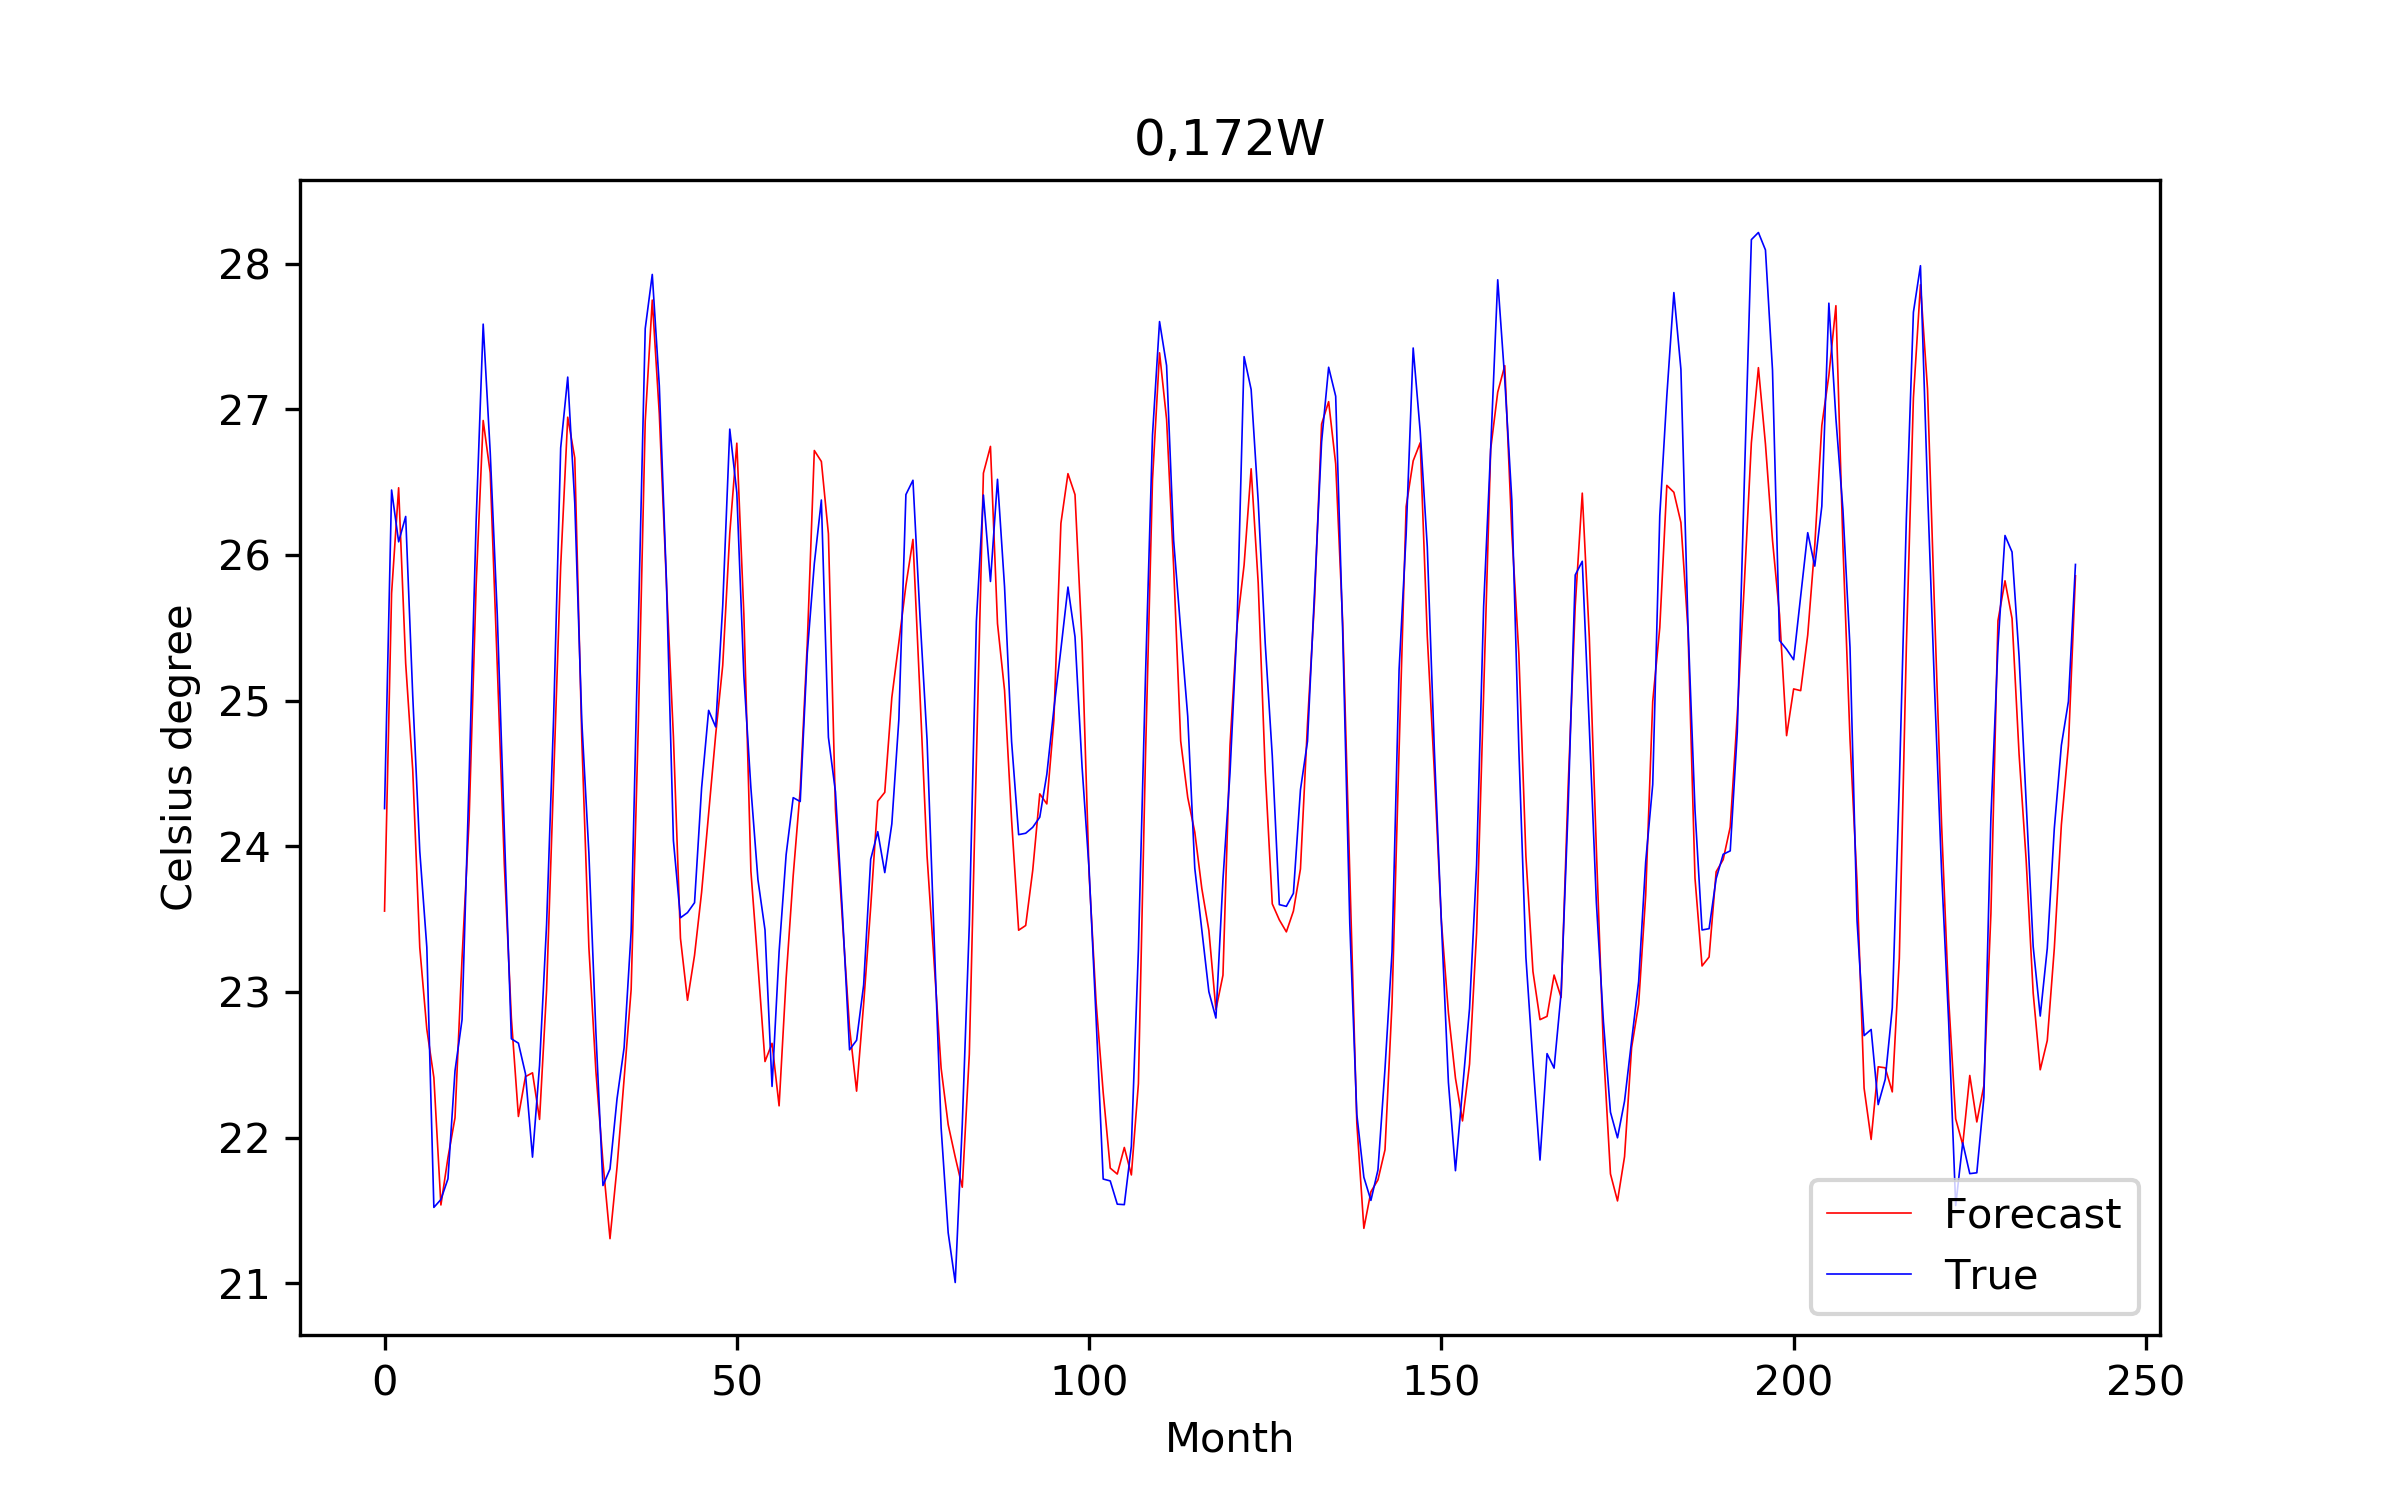
\includegraphics[width=0.4\textwidth]{0,172W.png}
        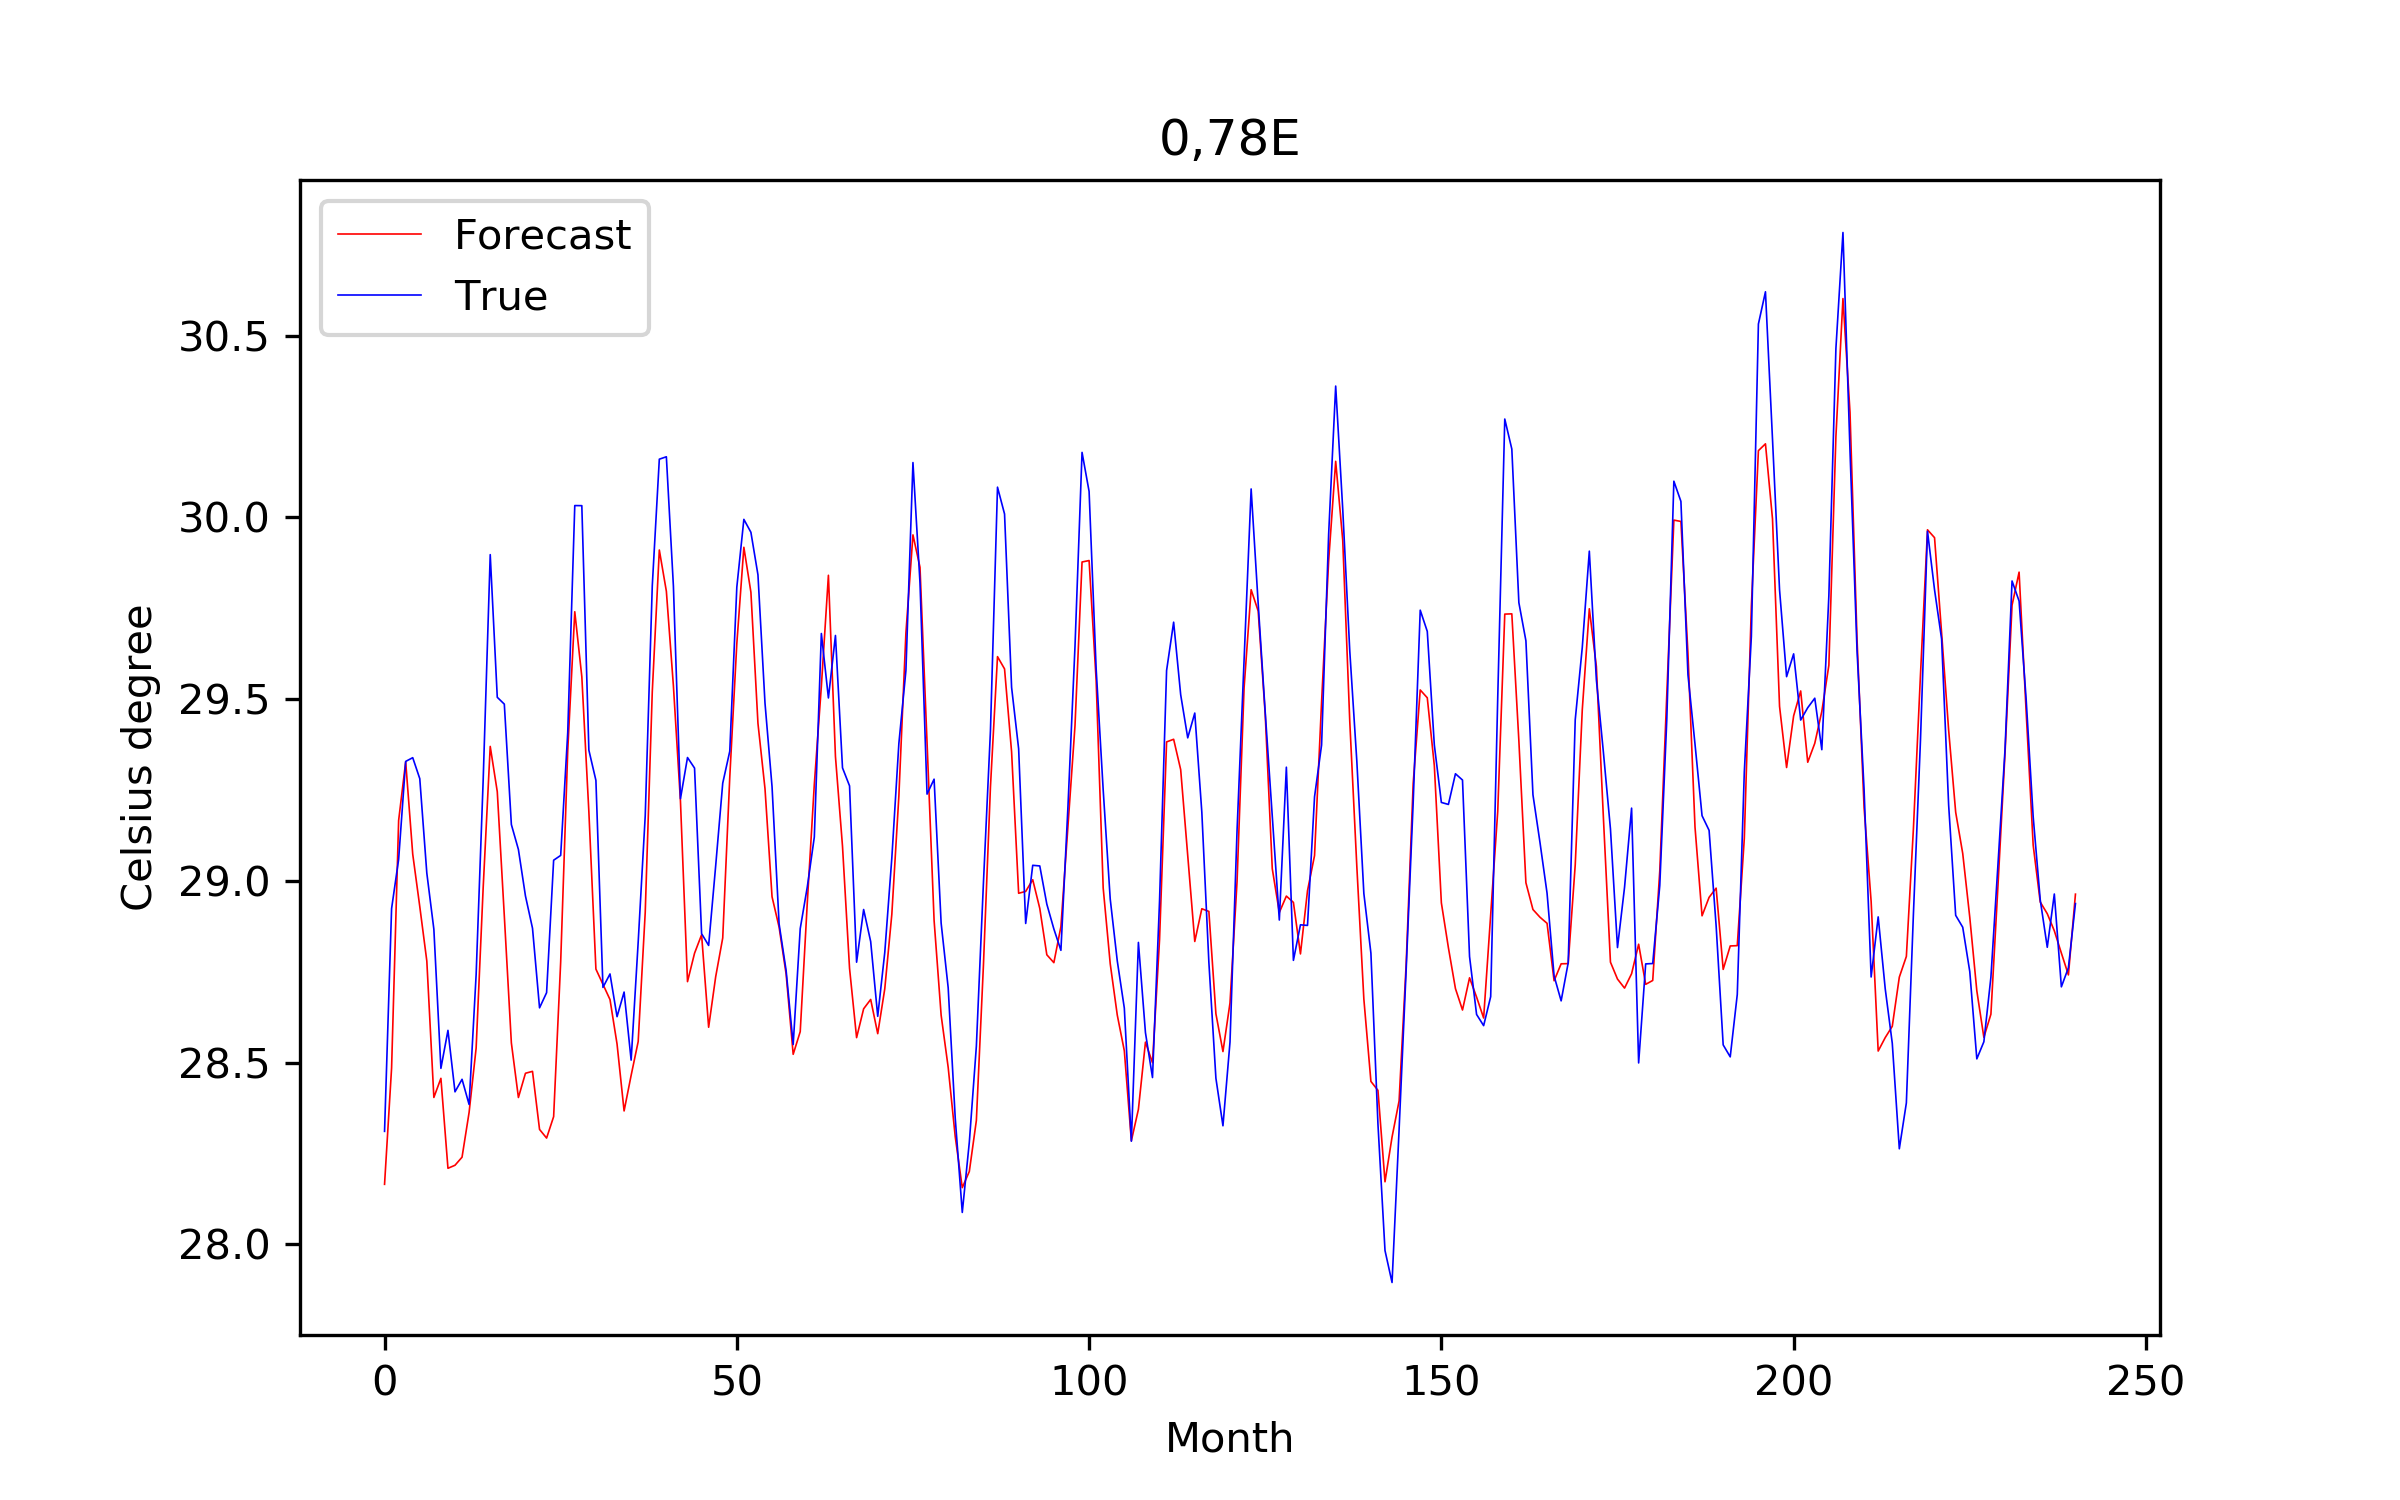
\includegraphics[width=0.4\textwidth]{0,78E.png}
        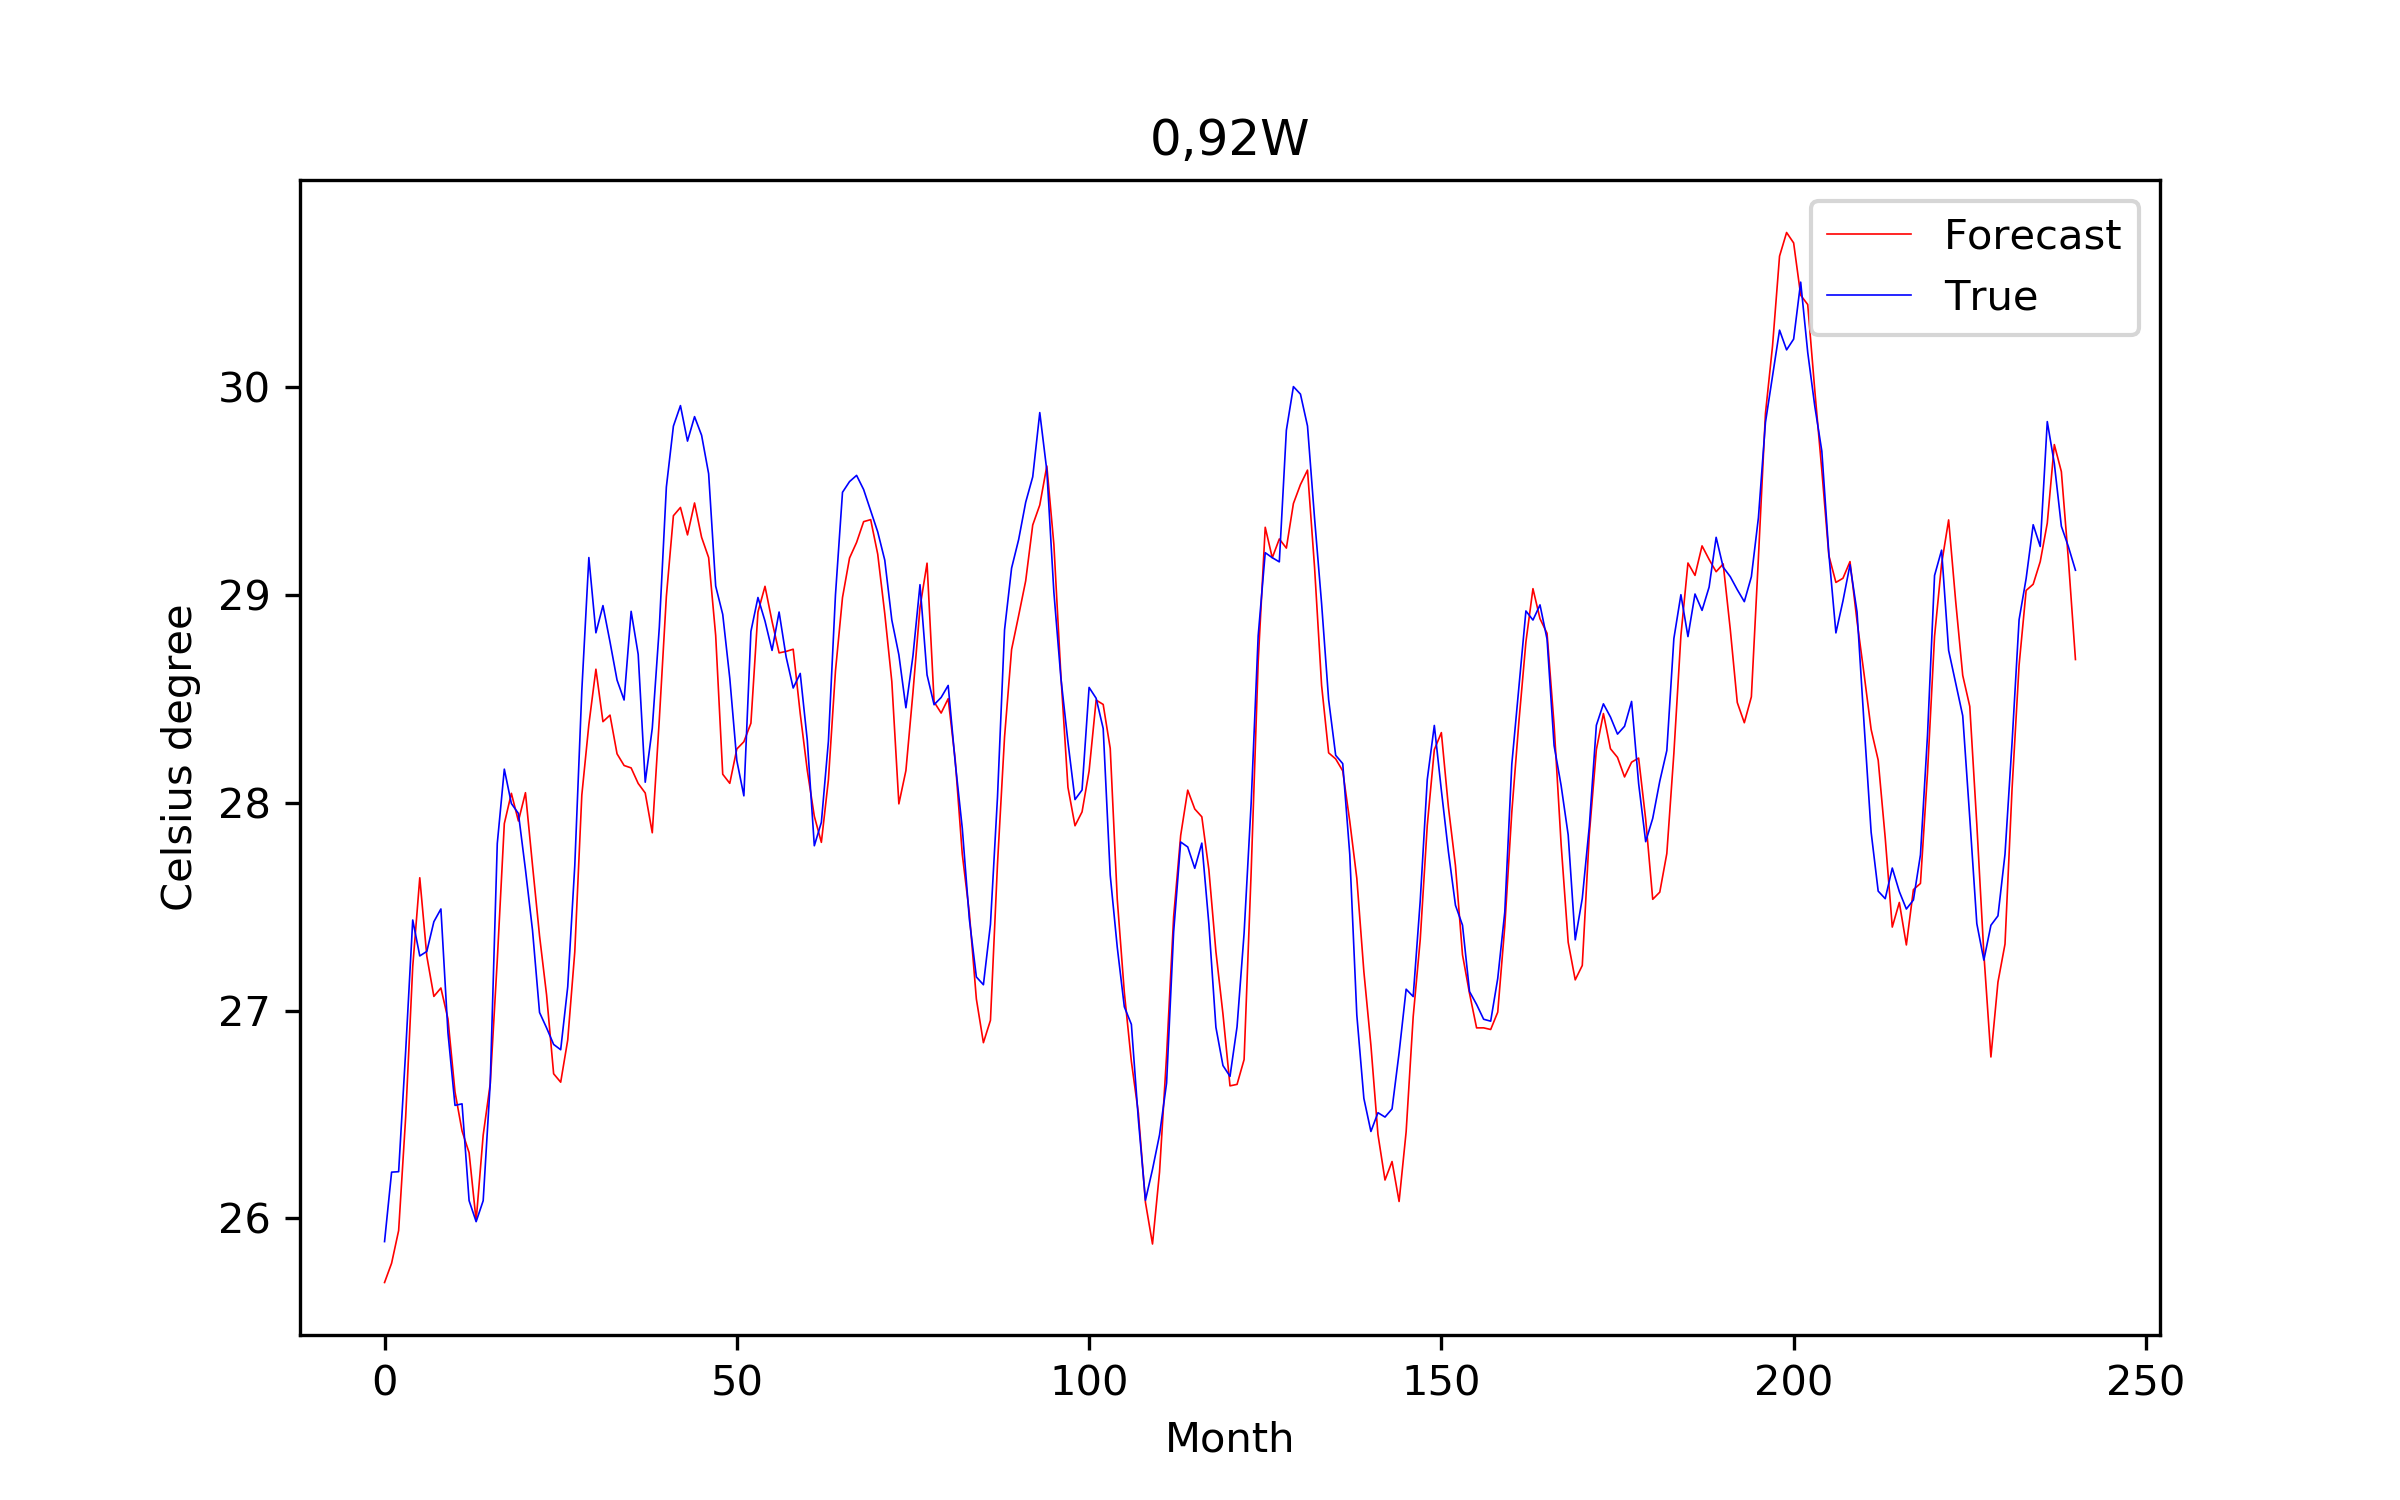
\includegraphics[width=0.4\textwidth]{0,92W.png}
        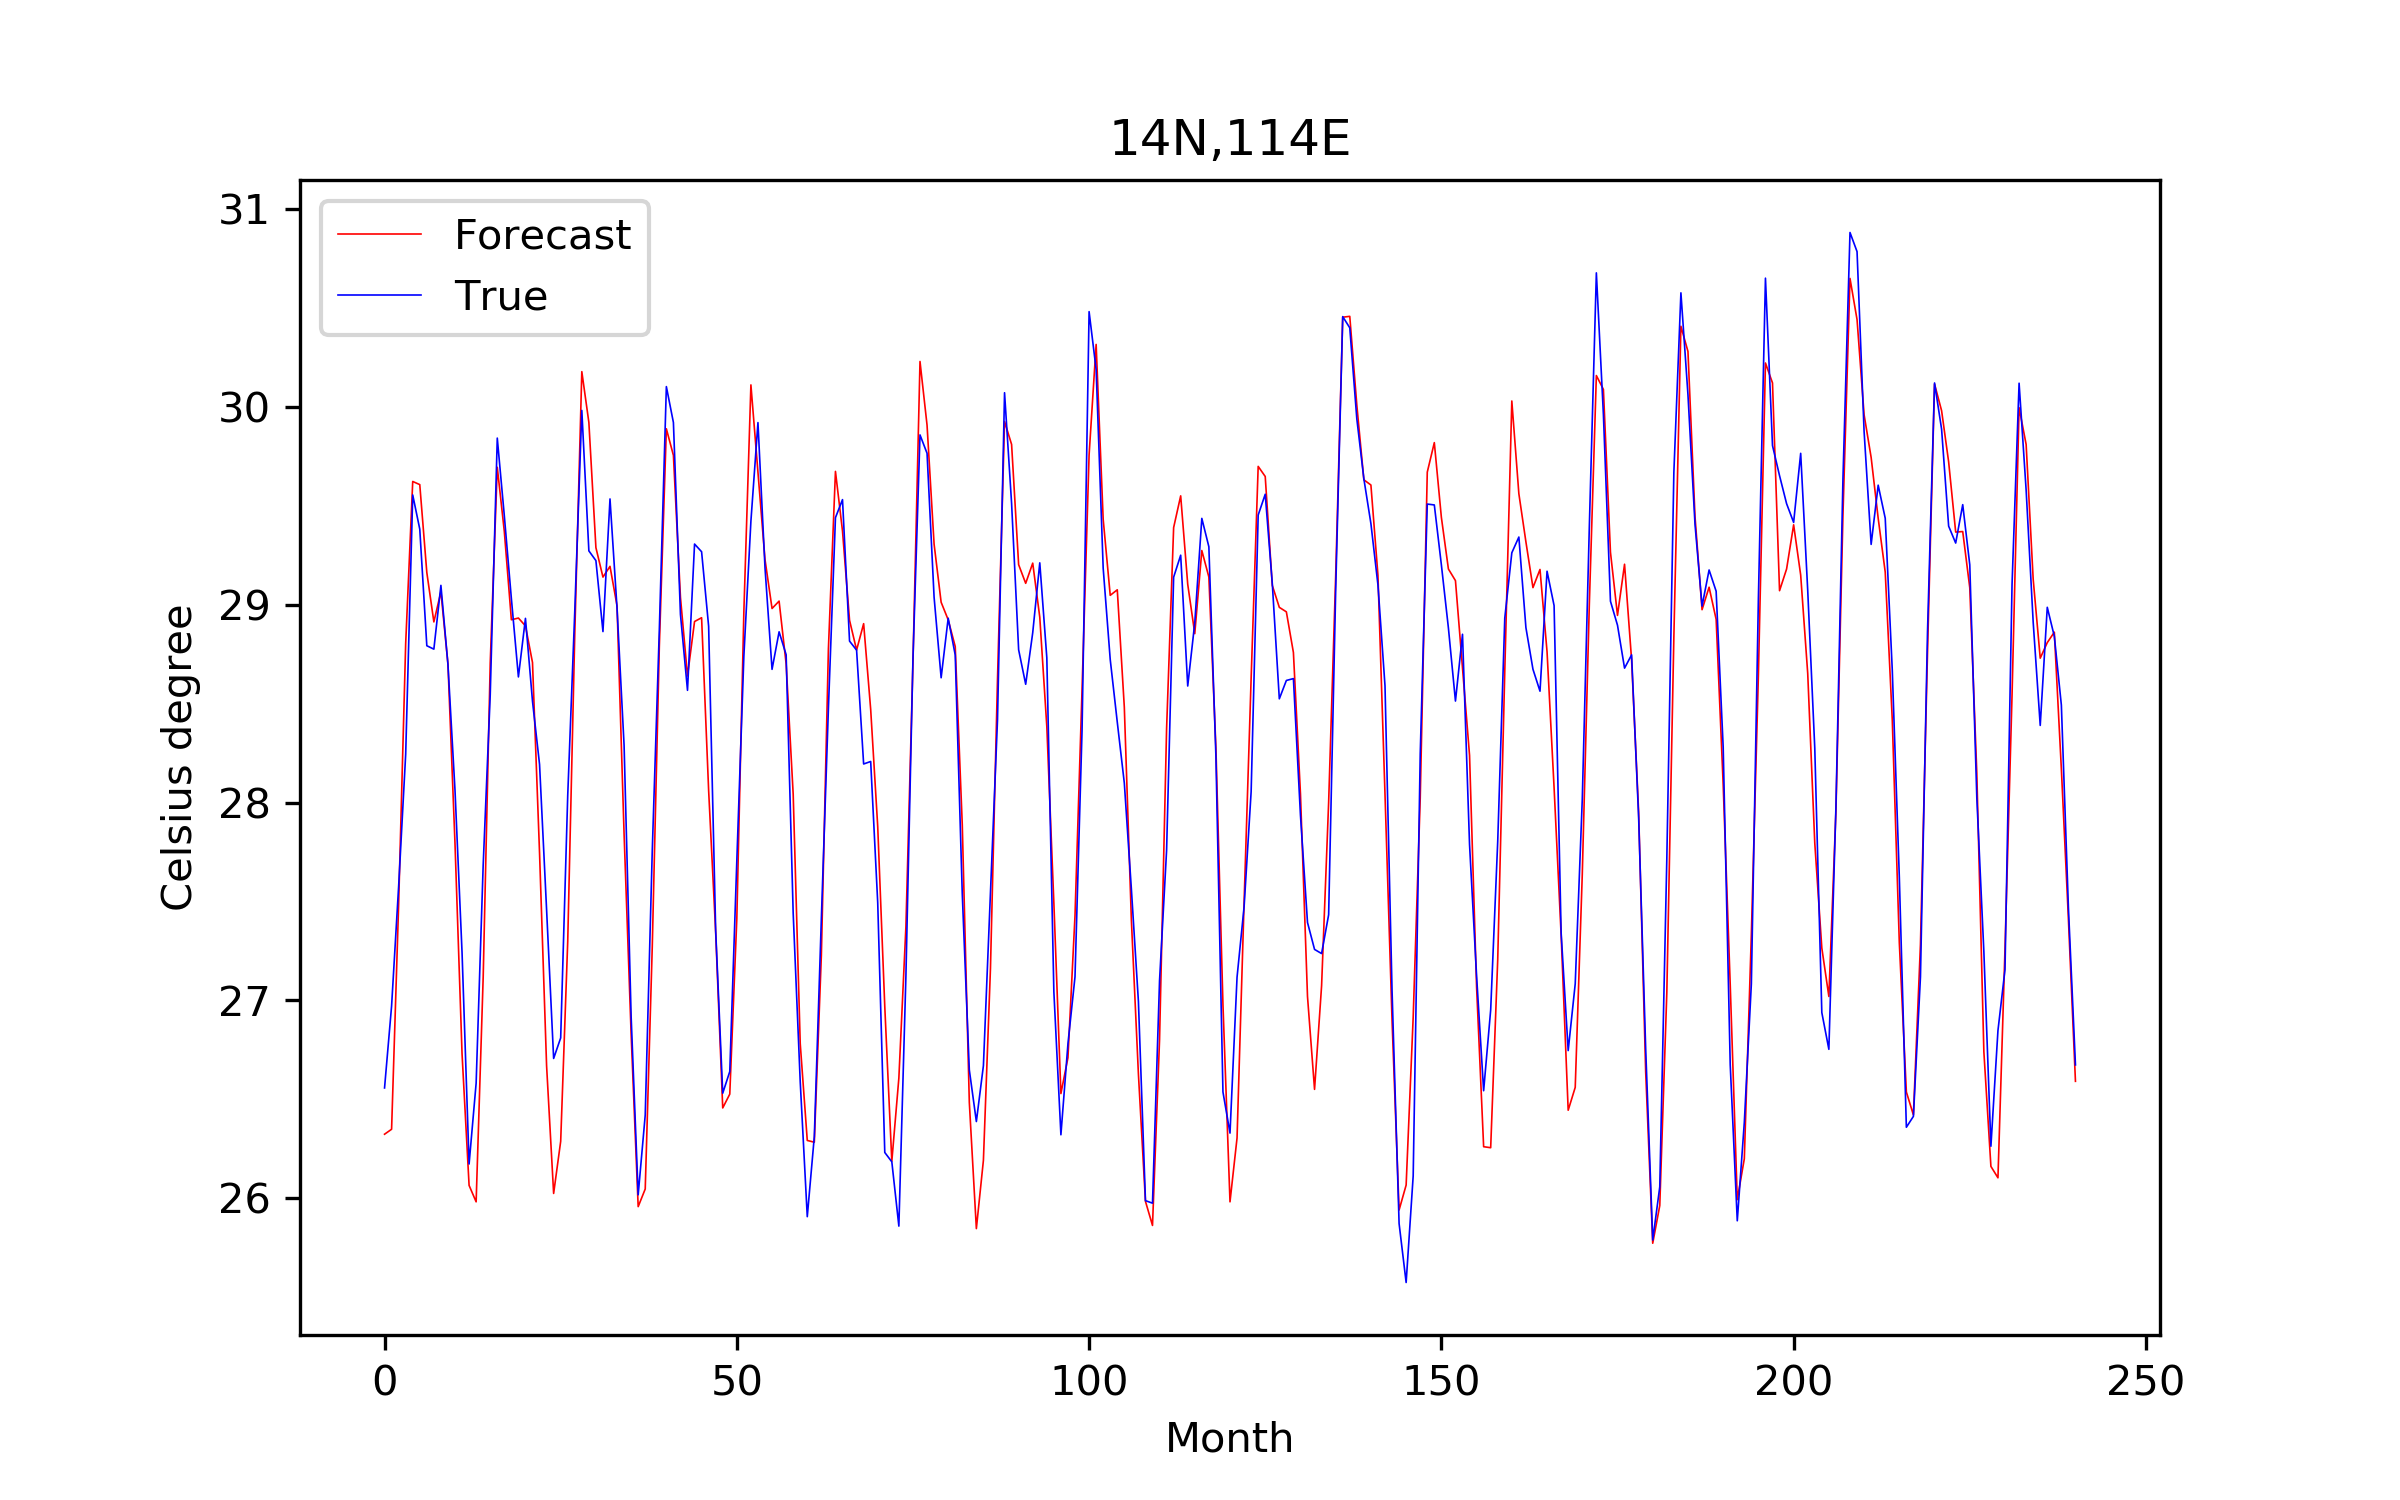
\includegraphics[width=0.4\textwidth]{14N,114E.png}
        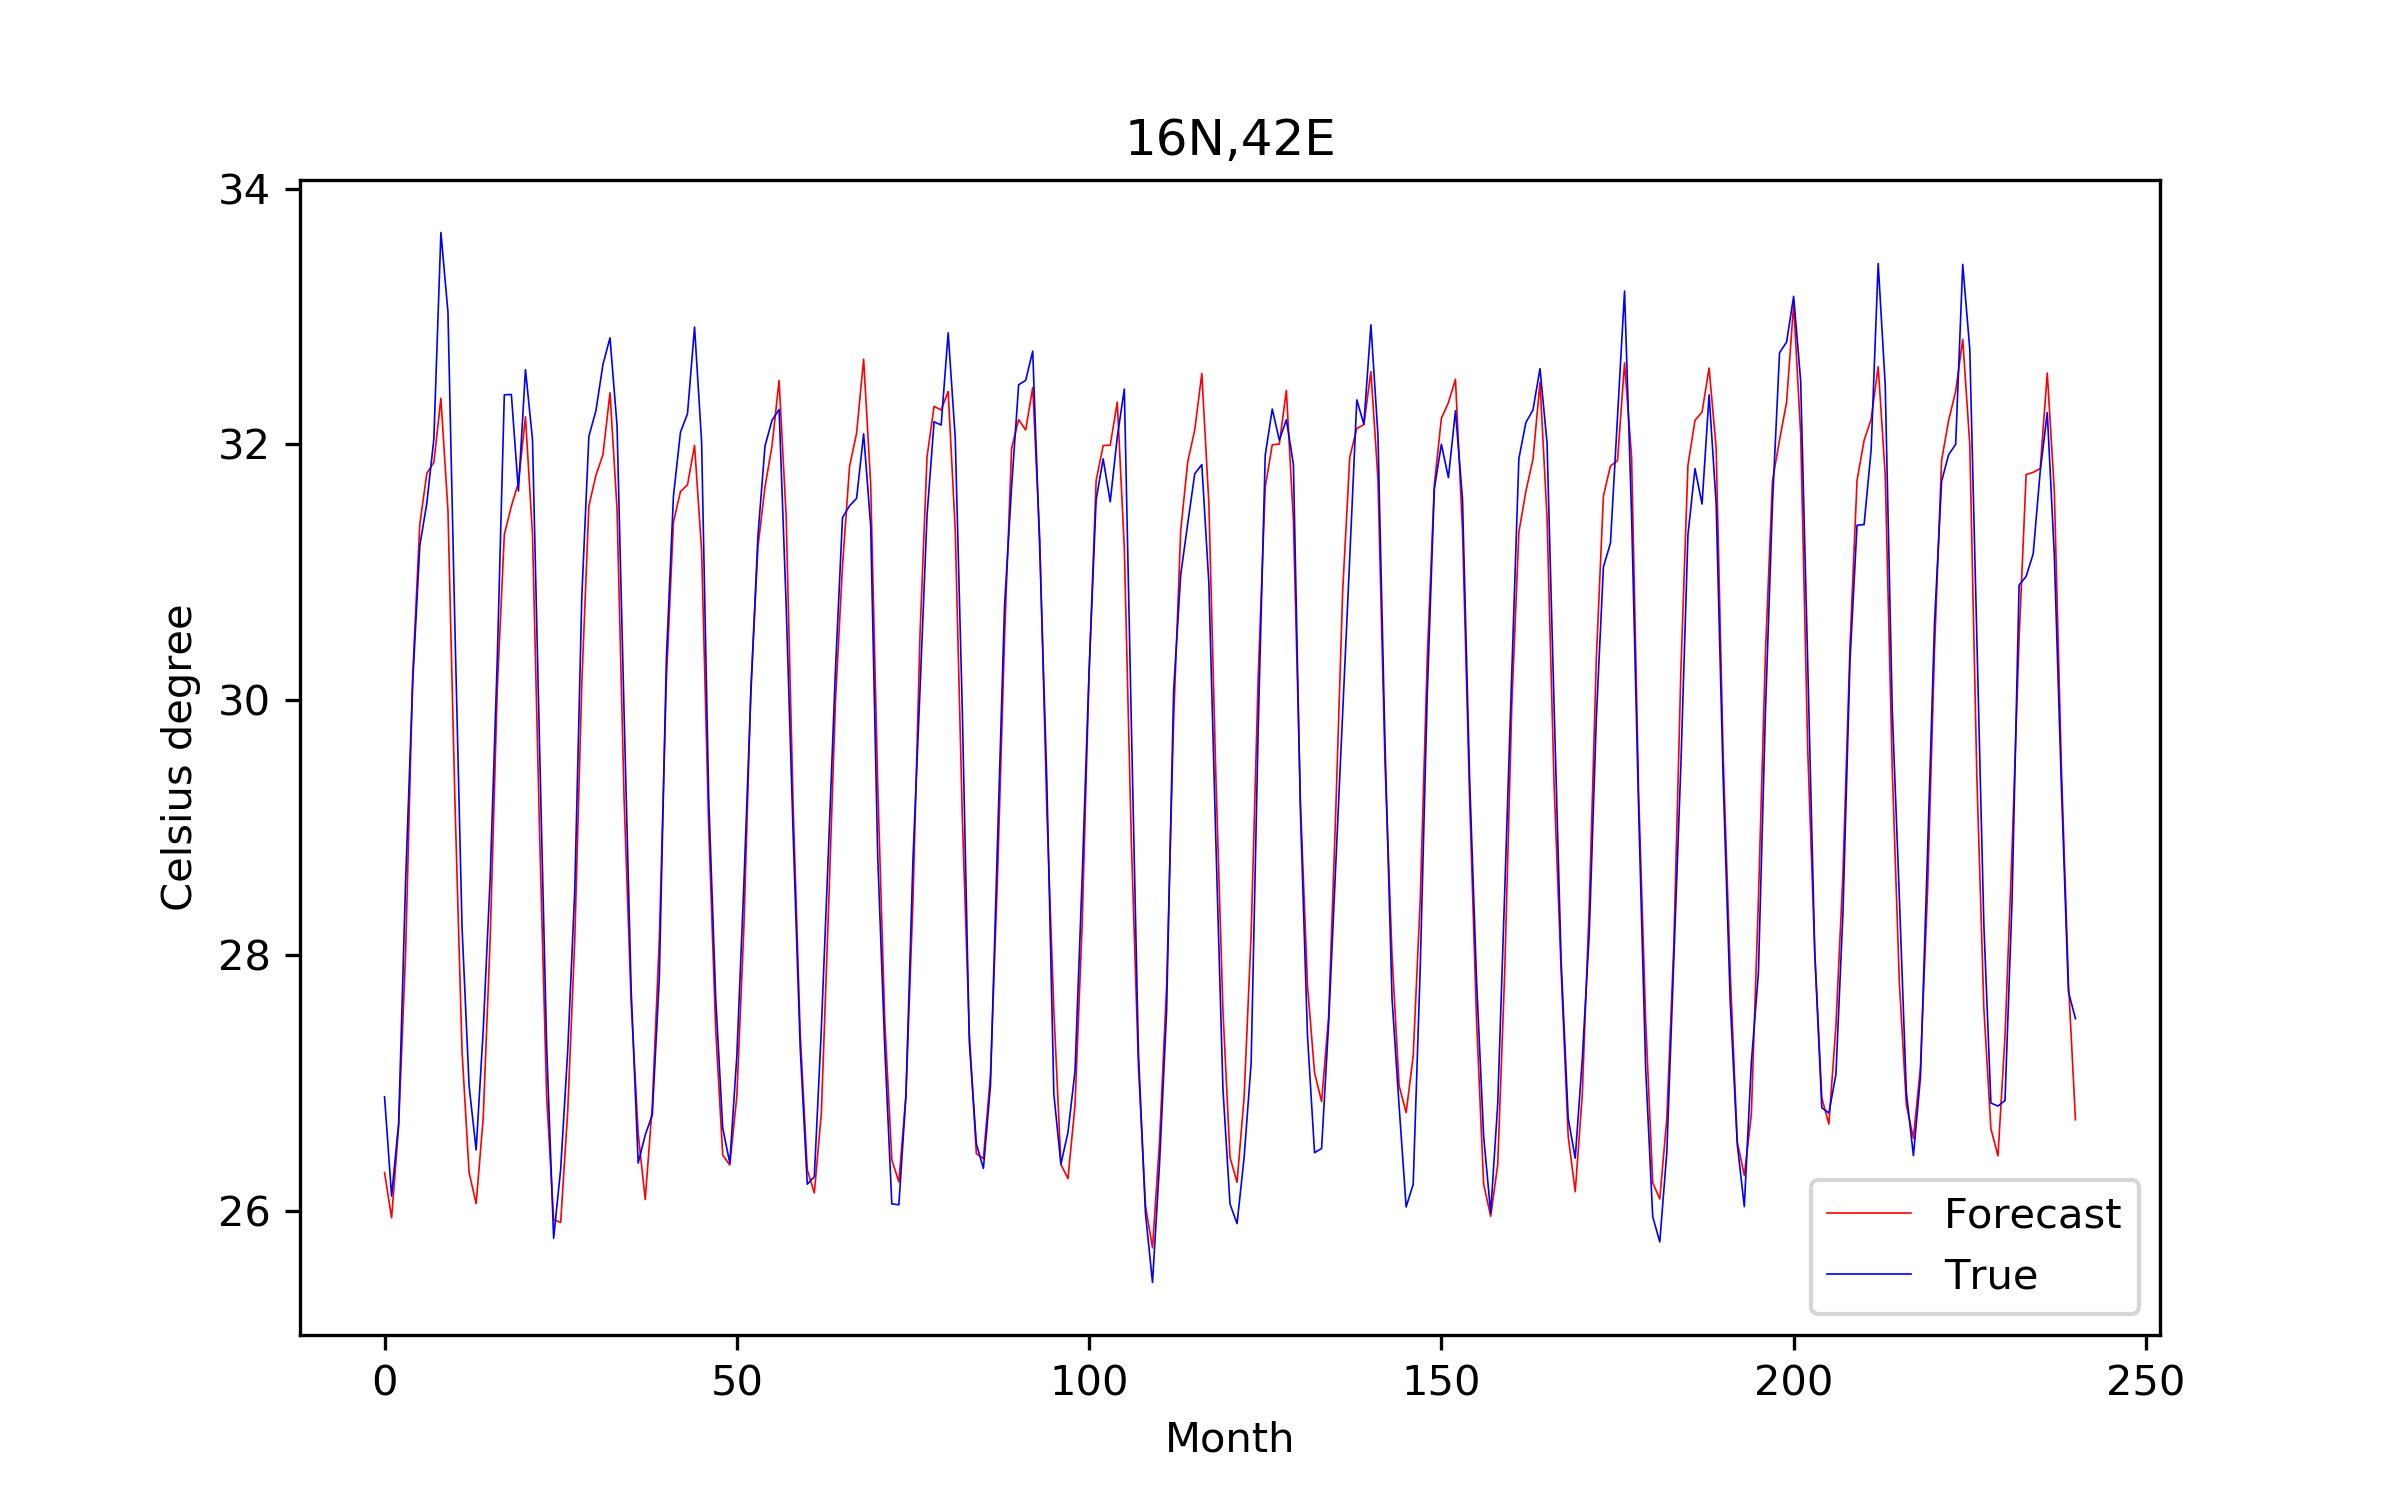
\includegraphics[width=0.4\textwidth]{16N,42E.png}
        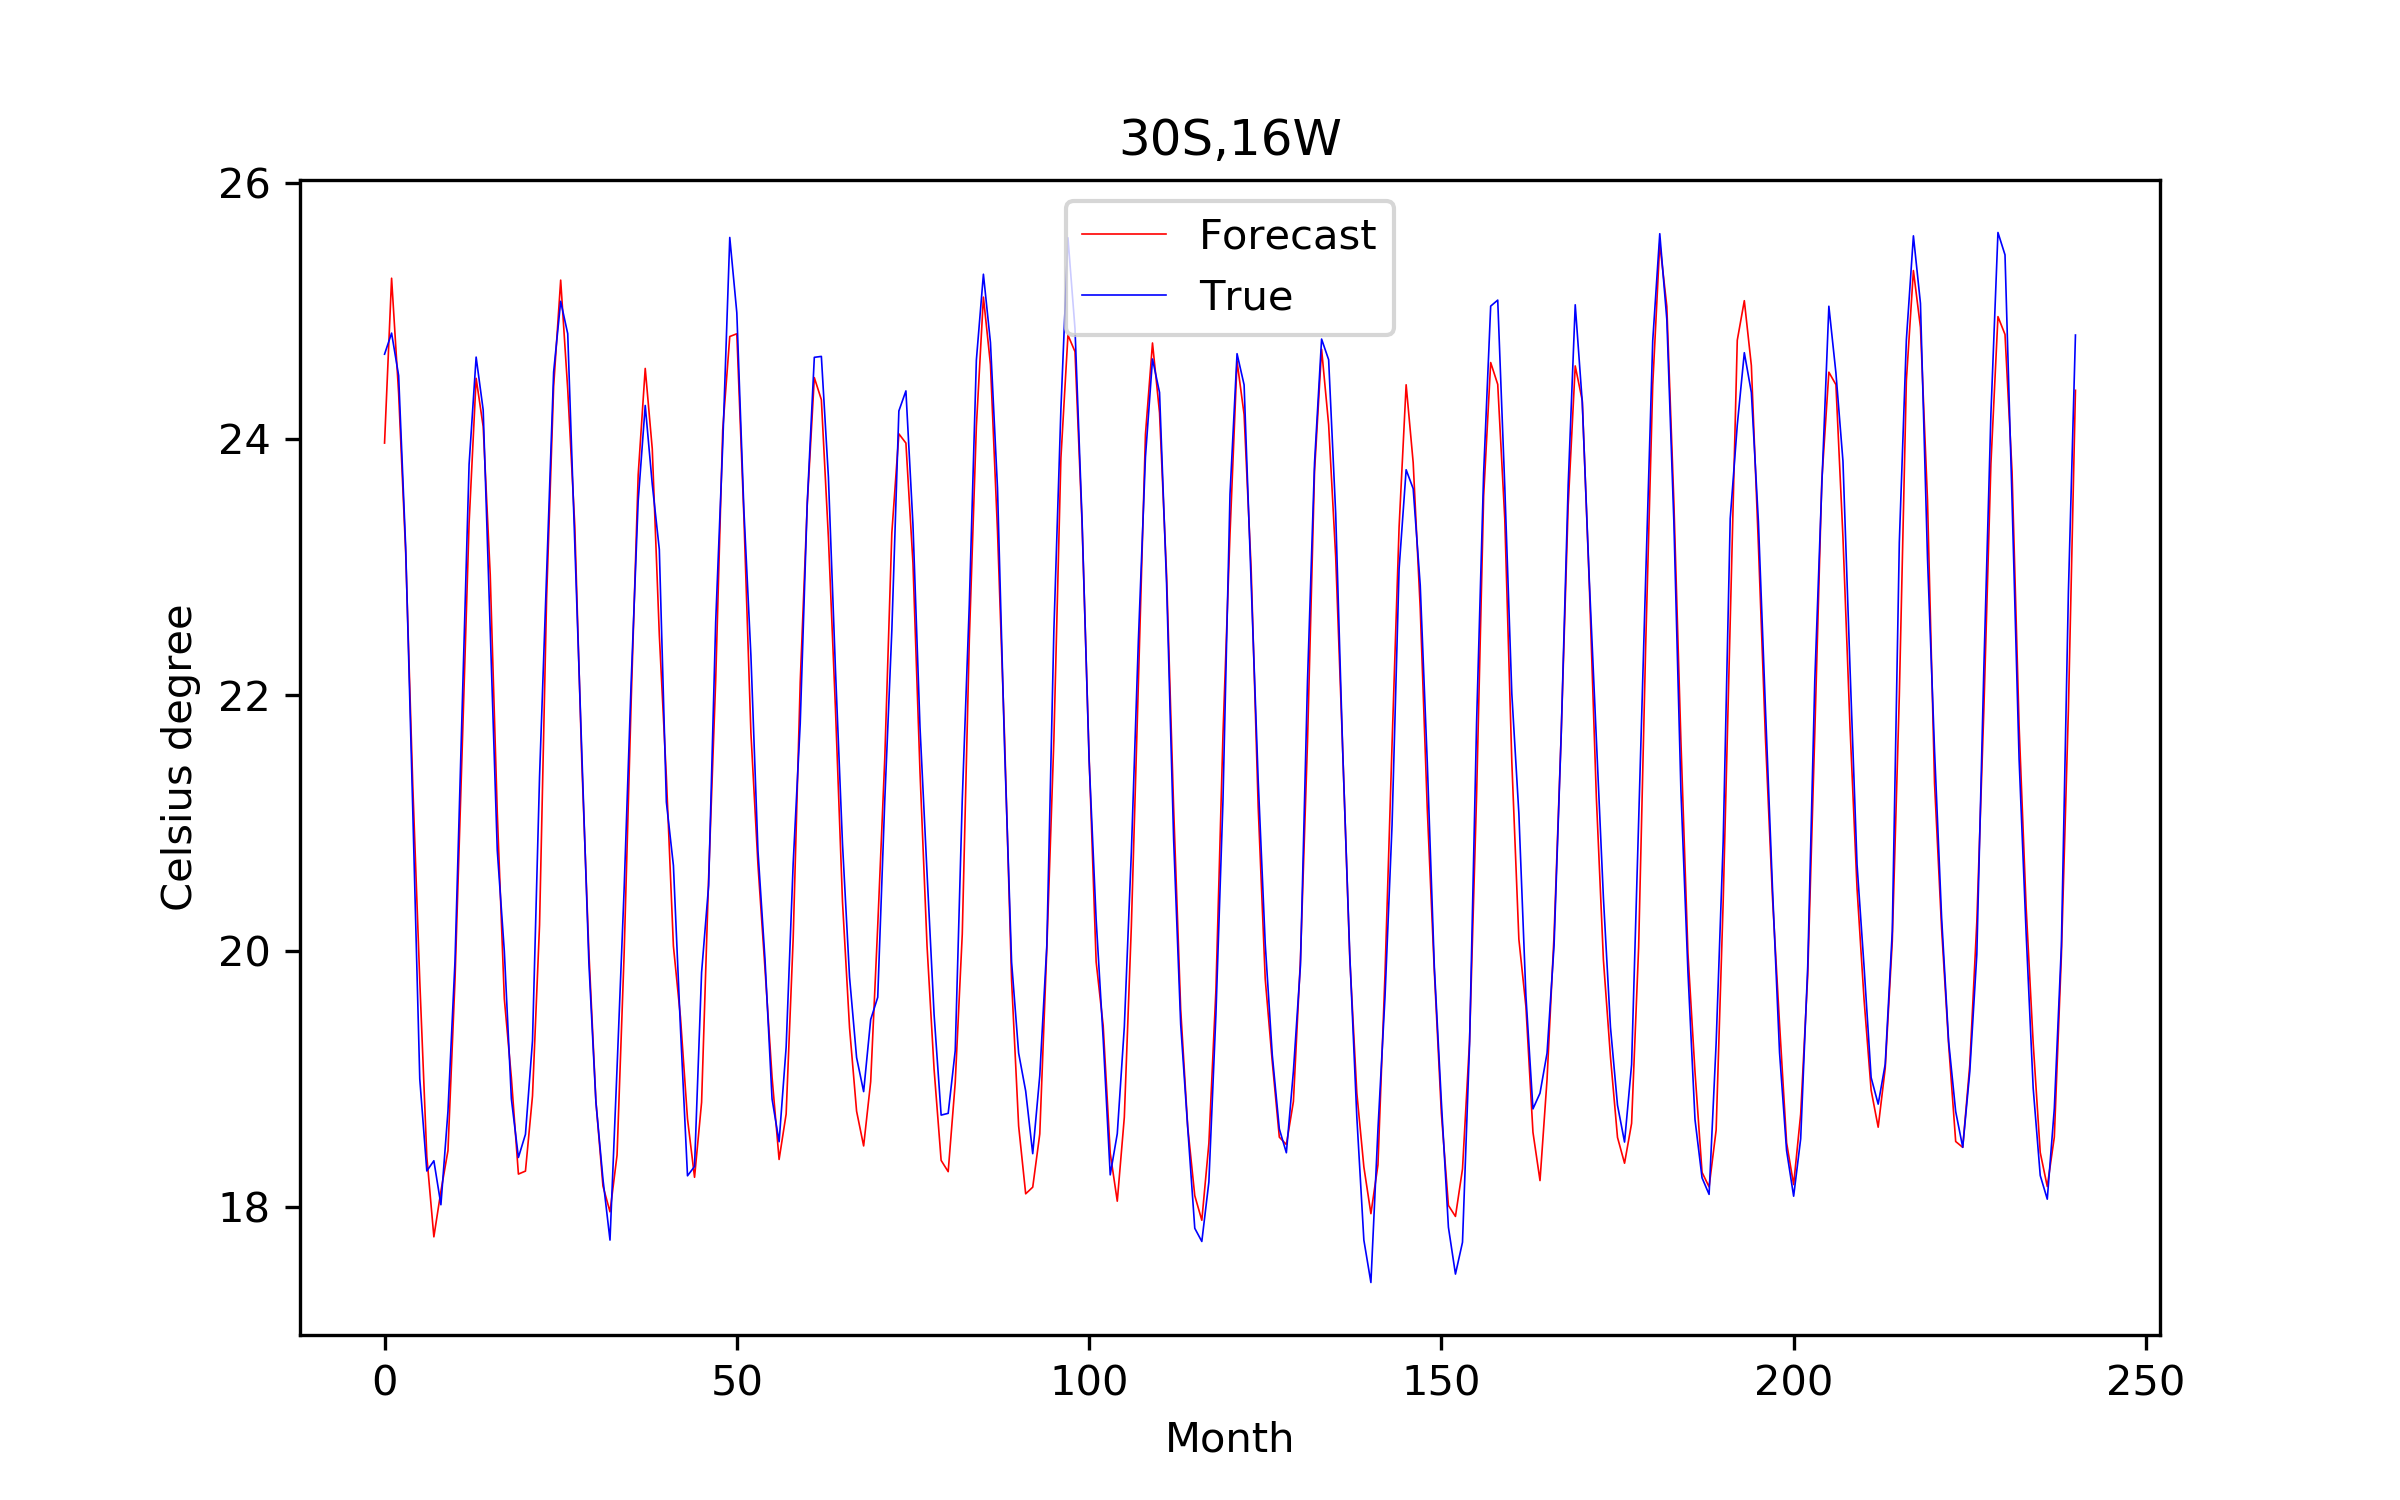
\includegraphics[width=0.4\textwidth]{30S,16W.png}
        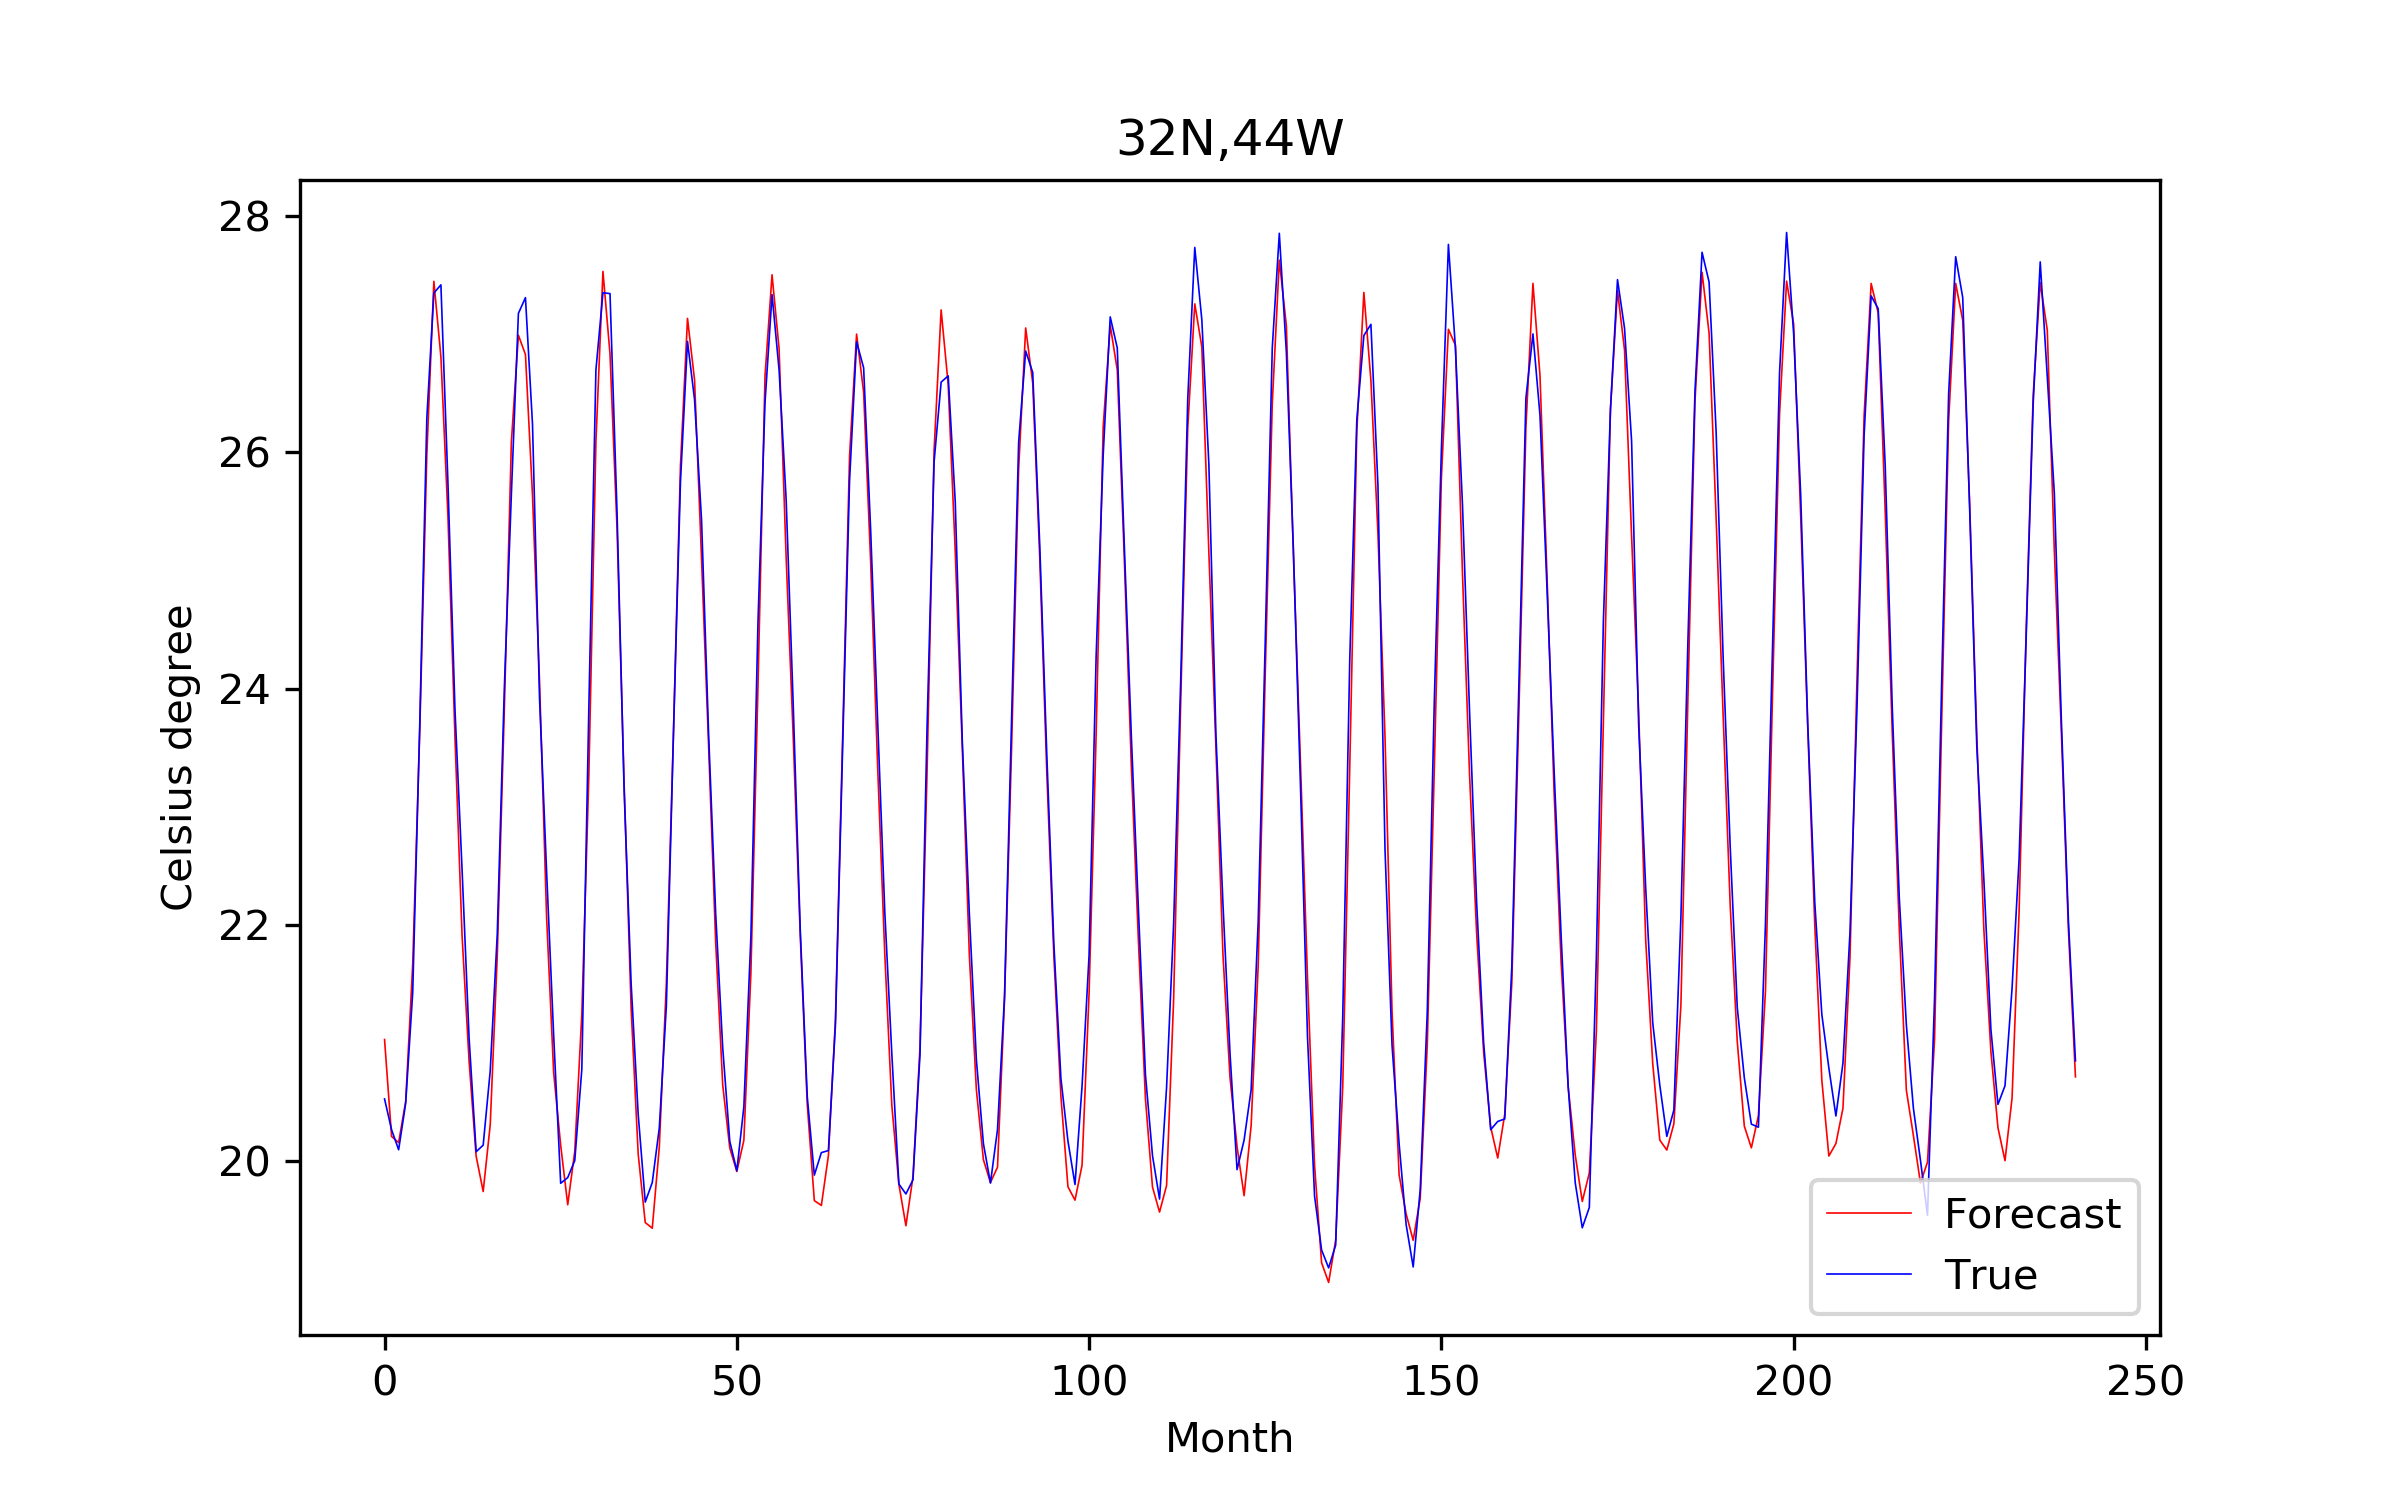
\includegraphics[width=0.4\textwidth]{32N,44W.png}
        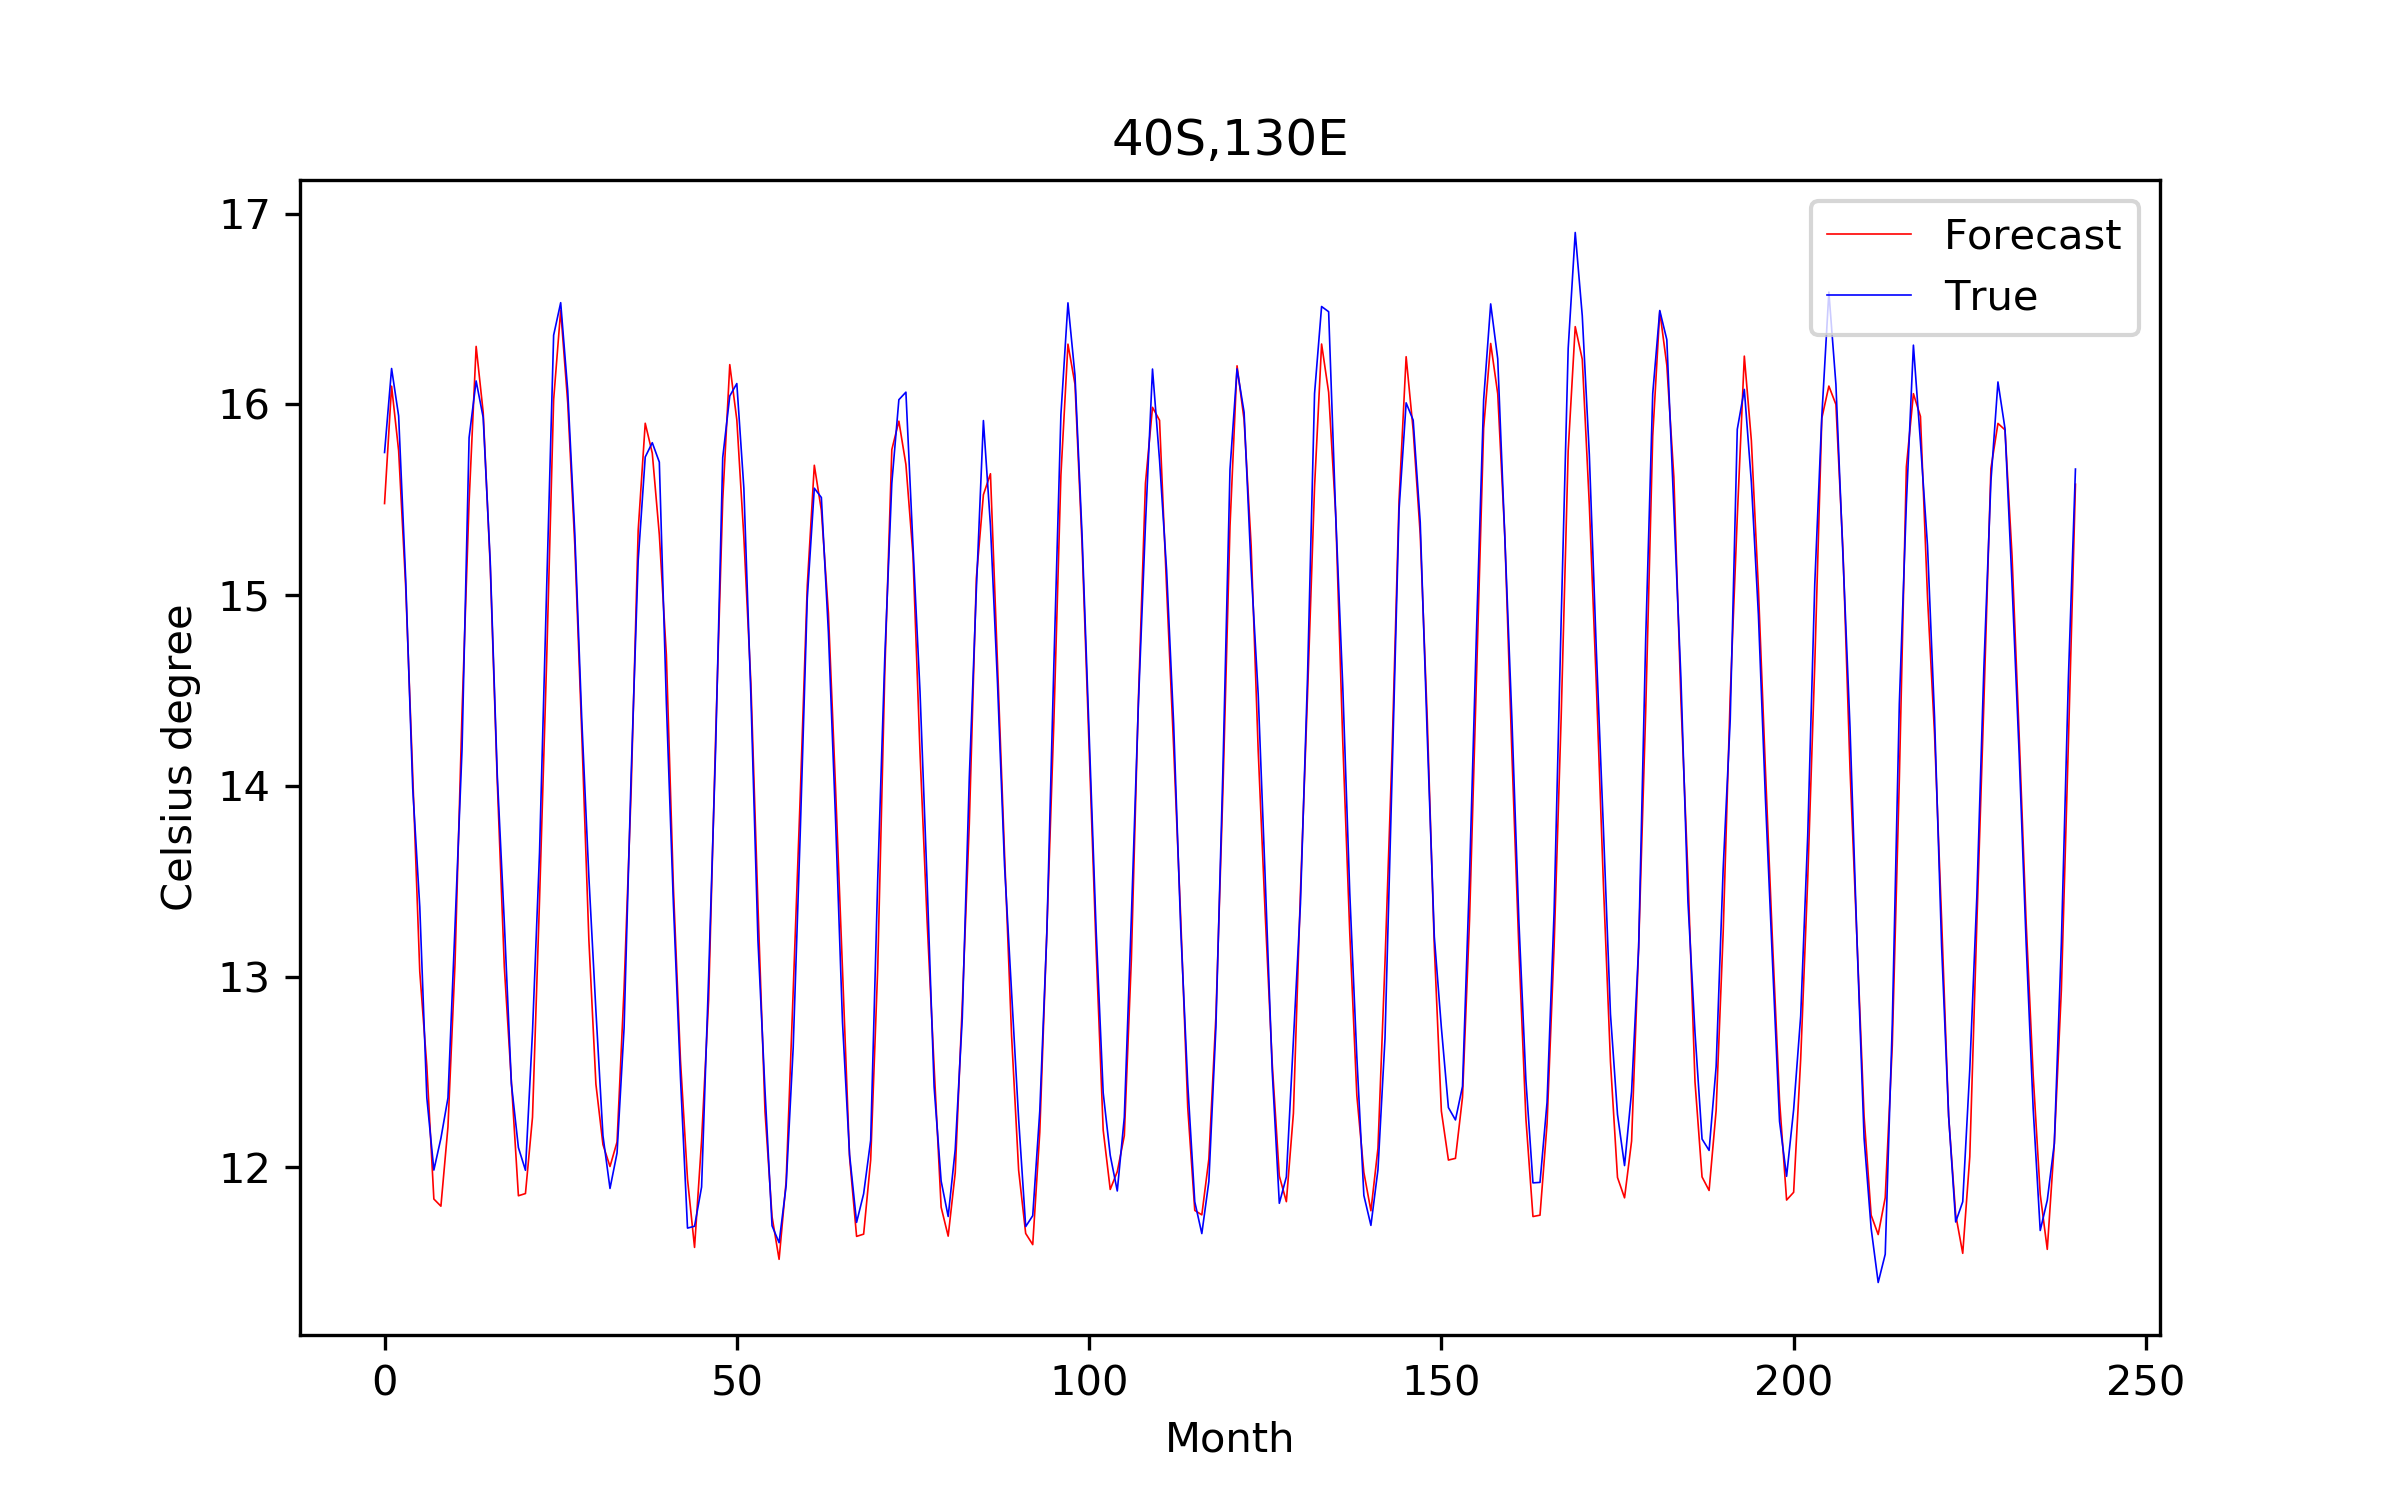
\includegraphics[width=0.4\textwidth]{40S,130E.png}
        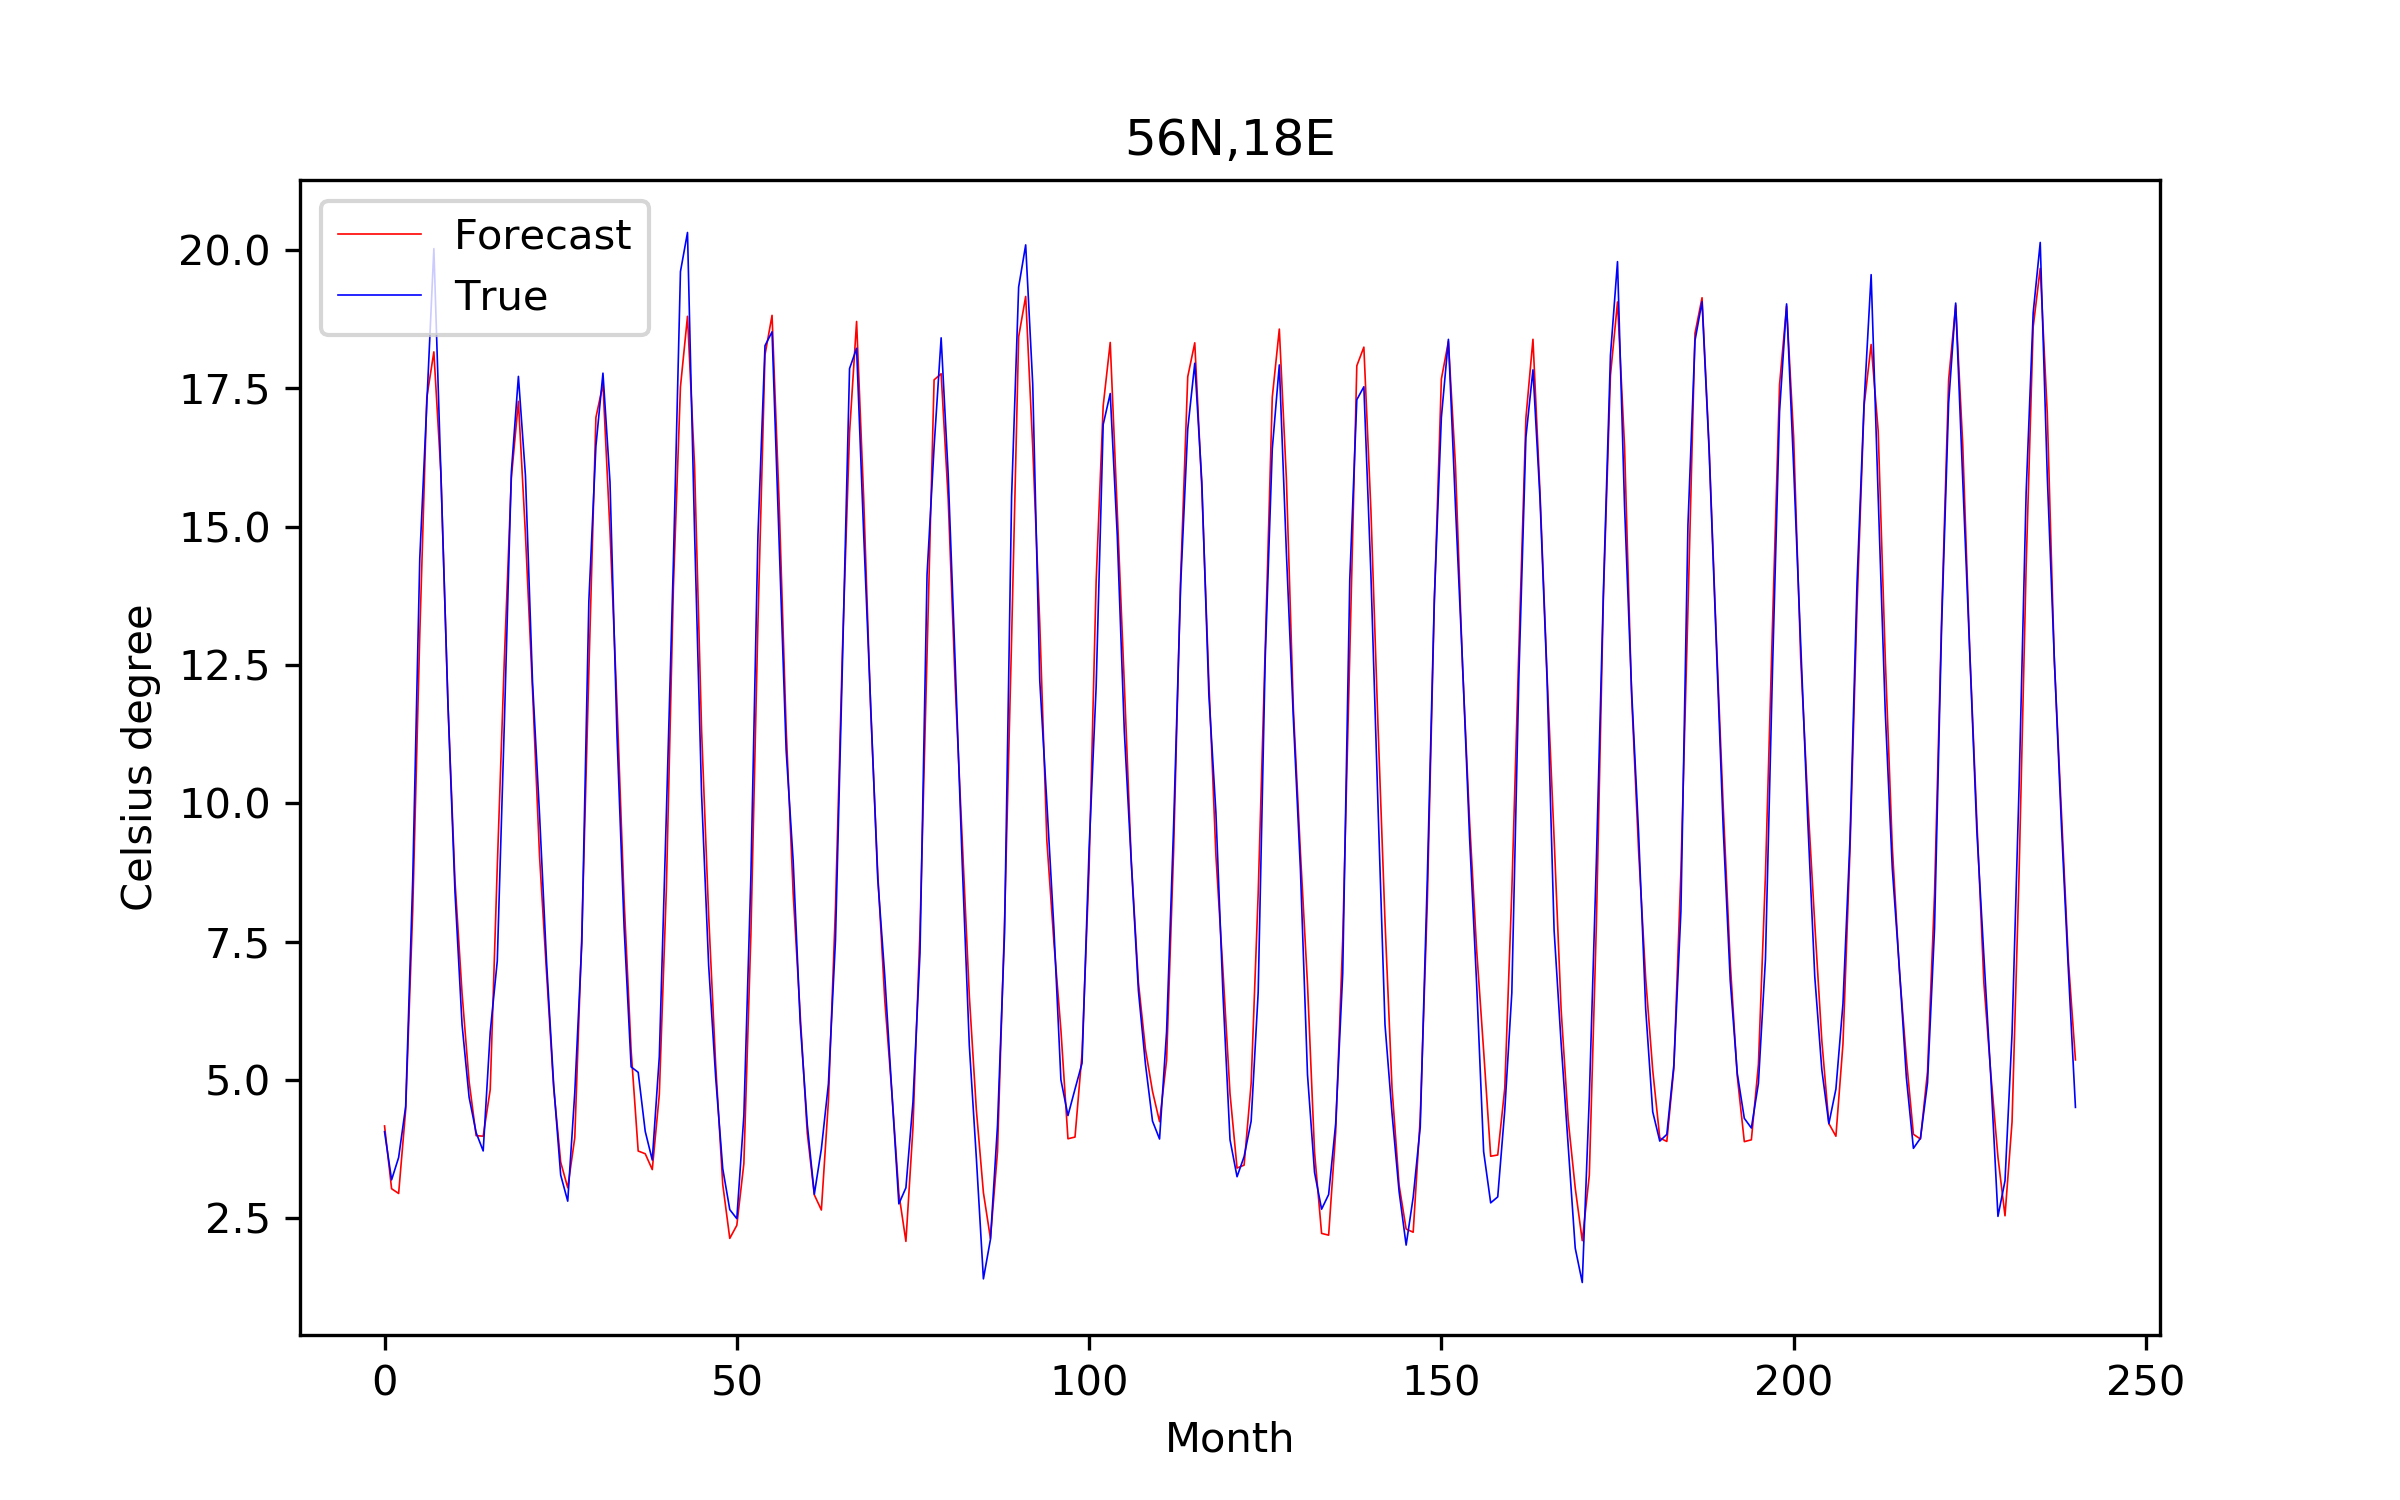
\includegraphics[width=0.4\textwidth]{56N,18E.png}
        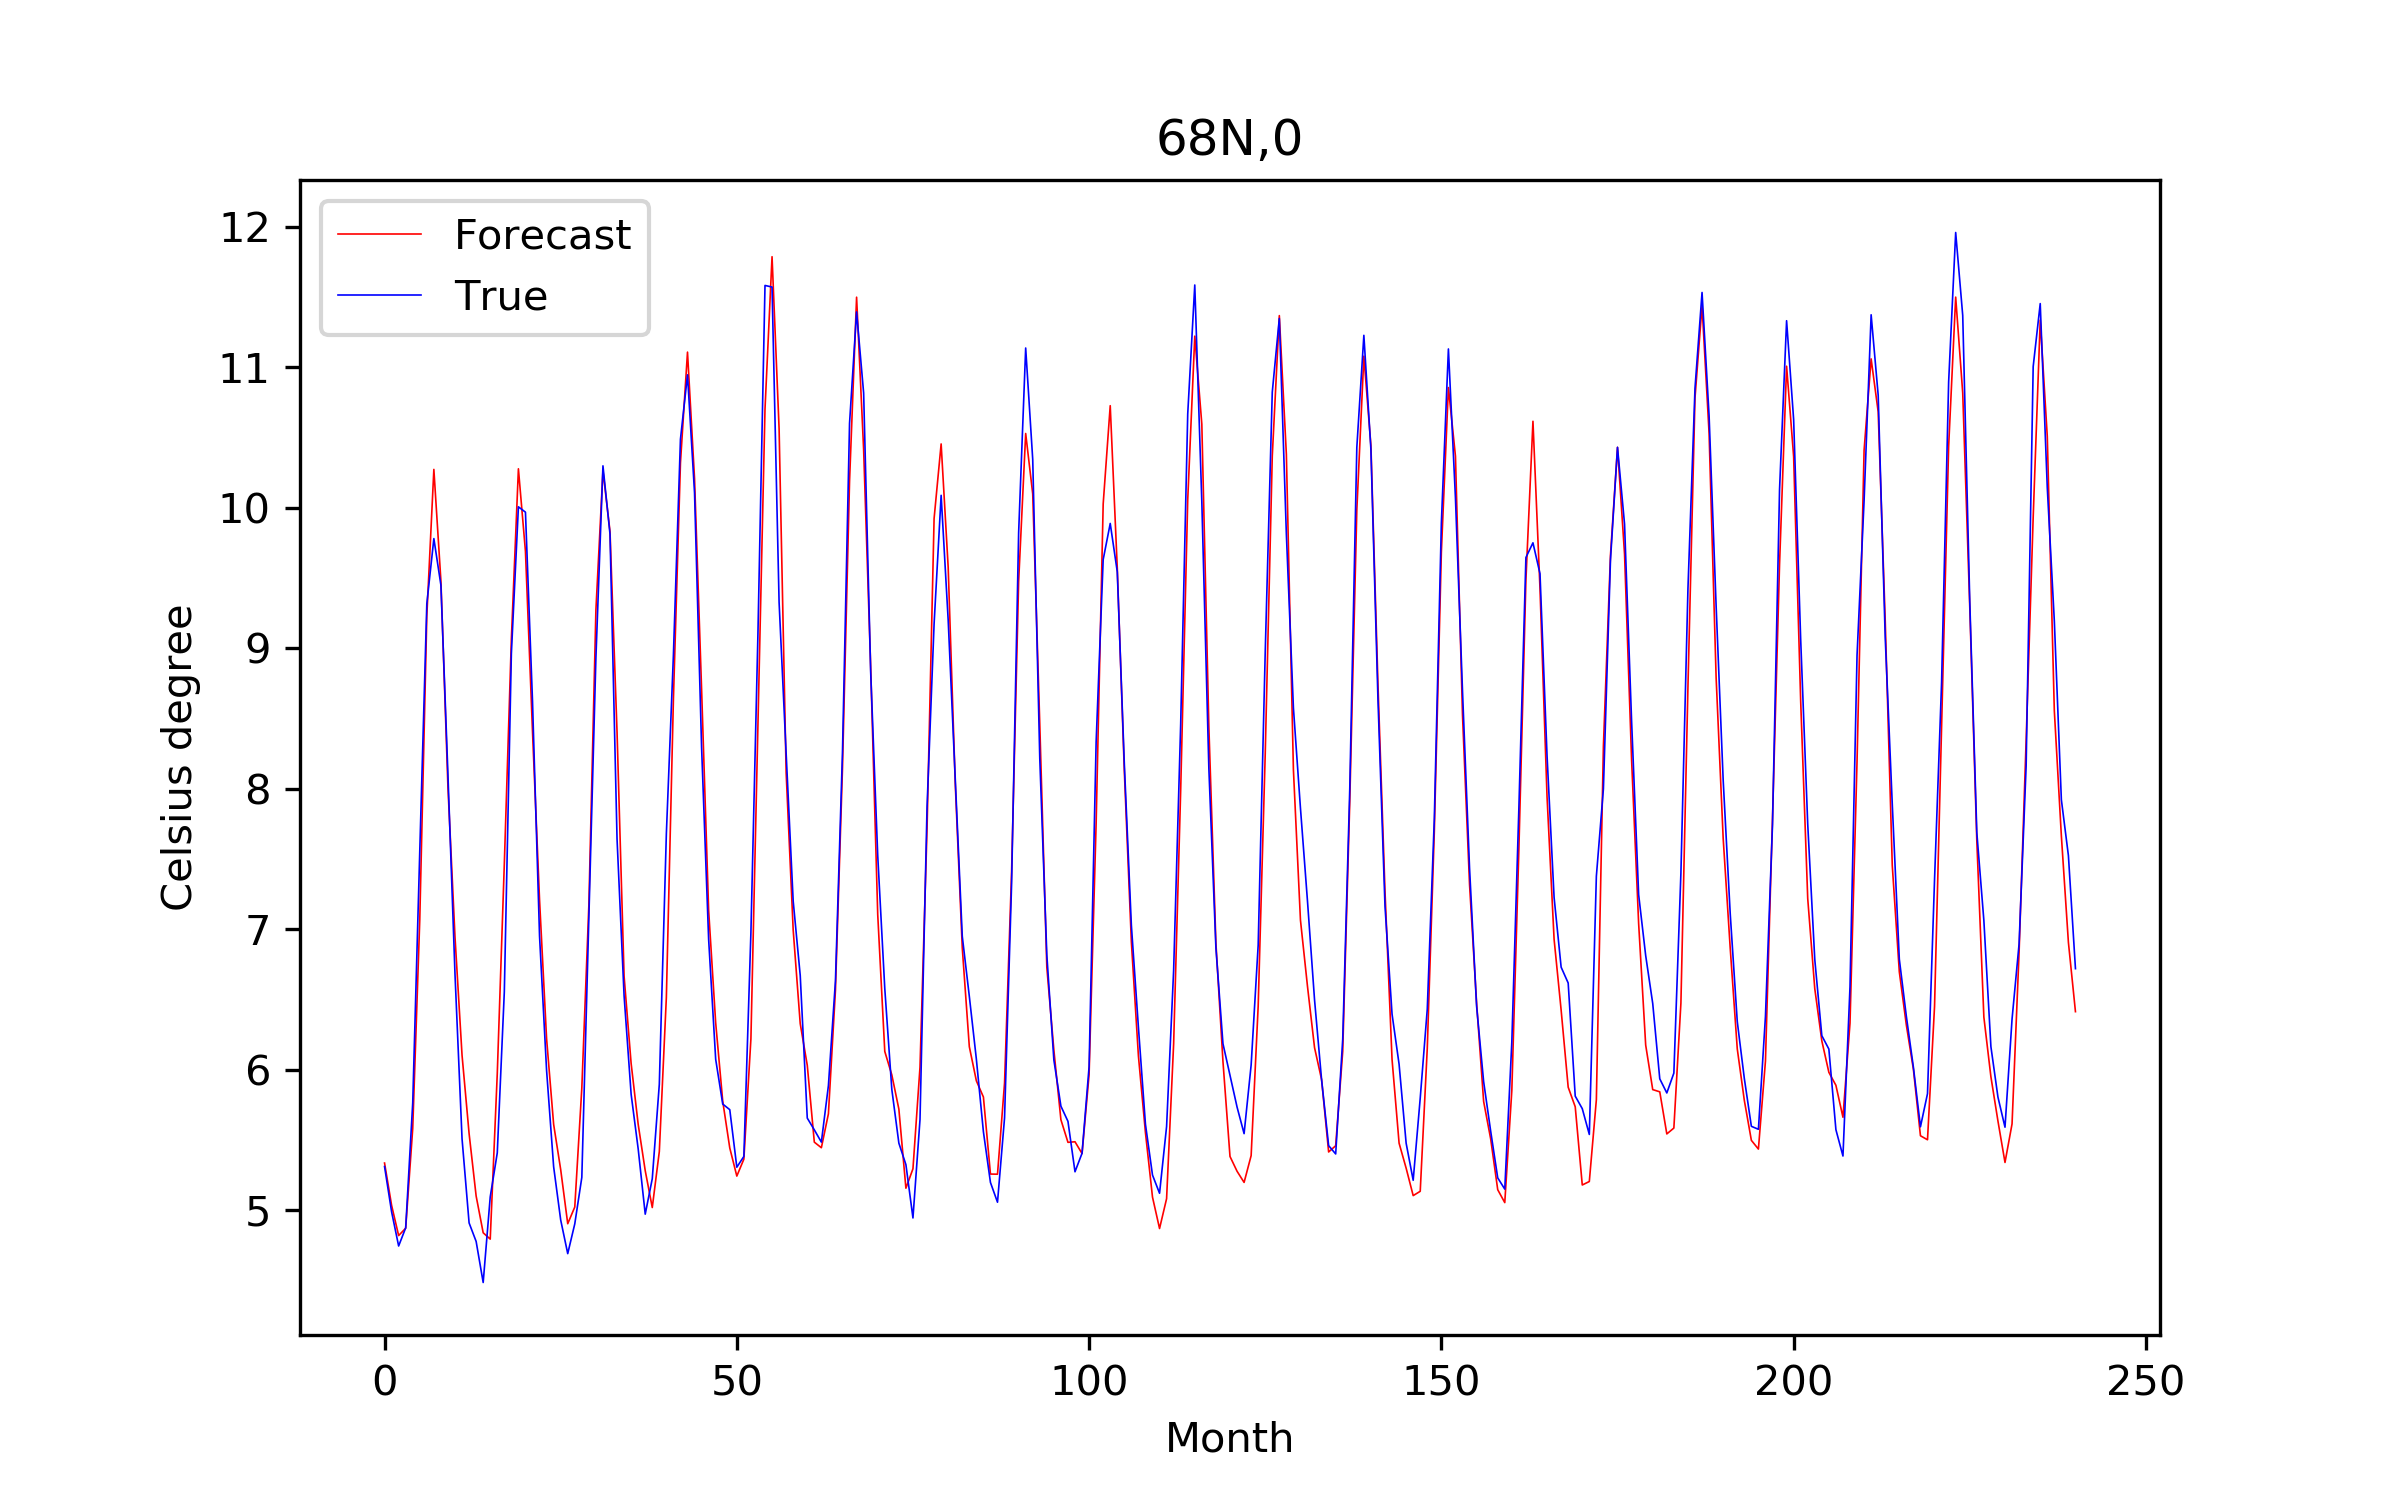
\includegraphics[width=0.4\textwidth]{68N,0.png}
    \end{figure}

    预测结果存储在Prediction.csv中,如下表所示:

    \begin{tabular}{|c|c|c|c|c|}
        \hline
        68N,0&56N,18E&32N,44W&16N,42E&14N,114E\\
        \hline
        5.86E+00&3.71E+00&1.98E+01&2.74E+01&2.77E+01\\
        \hline
        0,78E&0,92W&0,172W&30S,16W&40S,130E\\
        \hline
        2.98E+01&2.83E+01&2.73E+01&2.50E+01&1.58E+01\\
        \hline
    \end{tabular}

\end{document}